\documentclass[a4paper,french,12pt]{article}
\usepackage{babel,amssymb,amsmath}
\usepackage[utf8]{inputenc}
\usepackage{array,colortbl}
\usepackage[T1]{fontenc}
\usepackage{multicol}
%\usepackage{multirow}
%\usepackage[8pt]{pstricks}
\usepackage{textcomp}
\usepackage{fancyhdr}
\usepackage{geometry}
\usepackage{eurosym}
\usepackage{listings}
\usepackage{color}
\usepackage{placeins}
\usepackage{mathtools}
\definecolor{mygreen}{rgb}{0,0.6,0}
\definecolor{mygray}{rgb}{0.5,0.5,0.5}
\definecolor{mymauve}{rgb}{0.58,0,0.82}

\lstset{ %
  backgroundcolor=\color{white},   % choose the background color; you must add \usepackage{color} or \usepackage{xcolor}
  basicstyle=\footnotesize,        % the size of the fonts that are used for the code
  breakatwhitespace=false,         % sets if automatic breaks should only happen at whitespace
  breaklines=true,                 % sets automatic line breaking
  captionpos=b,                    % sets the caption-position to bottom
  commentstyle=\color{green},    % comment style
  deletekeywords={...},            % if you want to delete keywords from the given language
  escapeinside={\%*}{*)},          % if you want to add LaTeX within your code
  extendedchars=true,              % lets you use non-ASCII characters; for 8-bits encodings only, does not work with UTF-8
  frame=single,                    % adds a frame around the code
  keepspaces=true,                 % keeps spaces in text, useful for keeping indentation of code (possibly needs columns=flexible)
  keywordstyle=\color{blue},       % keyword style
  language=C++,                 % the language of the code
  morekeywords={*,...},            % if you want to add more keywords to the set
  numbers=left,                    % where to put the line-numbers; possible values are (none, left, right)
  numbersep=5pt,                   % how far the line-numbers are from the code
  numberstyle=\tiny\color{mygray}, % the style that is used for the line-numbers
  rulecolor=\color{black},         % if not set, the frame-color may be changed on line-breaks within not-black text (e.g. comments (green here))
  showspaces=false,                % show spaces everywhere adding particular underscores; it overrides 'showstringspaces'
  showstringspaces=false,          % underline spaces within strings only
  showtabs=false,                  % show tabs within strings adding particular underscores
  stepnumber=1,                    % the step between two line-numbers. If it's 1, each line will be numbered
  stringstyle=\color{mymauve},     % string literal style
  tabsize=2,                       % sets default tabsize to 2 spaces
  title=\lstname                   % show the filename of files included with \lstinputlisting; also try caption instead of title
}
% \usepackage{titling}
%\usepackage{makeidx}
% \usepackage[maxfloats=50]{morefloats}
% \usepackage{hyperref}
\usepackage{ulem}

\usepackage{epigraph}
\geometry{rmargin=2.5cm, lmargin=2.5cm, hmargin=2cm, bmargin=2cm}
\pagestyle{plain}
\usepackage[pdftex]{thumbpdf}
%\definecolor{vert}{rgb}{0.25,0.65,0.04}
\usepackage[pdftex,
    bookmarks         = true,
    bookmarksnumbered = true,
    pdfpagemode       = None,
    pdfstartview      = FitH,
    pdfpagelayout     = SinglePage,
    colorlinks        = true,
    linkcolor	      = black,
    pdfborder         = {0 0 0}
    ]{hyperref}
\usepackage{graphicx}
\usepackage[ruled]{algorithm2e}

\newcommand{\HRule}{\rule{\linewidth}{0.5mm}}
% \hypersetup{
% 	pdfauthor = {Philippe \textsc{GAULTIER}},
% 	pdftitle = {Rapport de stage du 17/06/2013 au 23/08/2013},
% 	pdfsubject = {},
% 	pdfkeywords = {},
% 	pdfcreator = {},
% }
% \newcommand{\filename}[1]{\textbf{\#1}}
% \newcommand{\fonction}[1]{\textbf{\itshape{\#1}}} 
% \newcommand{\tabl}[1]{\textbf{\itshape{\#1}}[ ]} 
\begin{document}
\begin{titlepage}
\begin{center}

%Logo

\includegraphics[width=0.4\textwidth]{./logo_ENSIIE.png}~\\[1cm]
\textsc{\huge Ensiie Strasbourg}\\[1.5cm]

%Title
\HRule \\[0.4cm]
{
	\huge \bfseries Rapport de stage
\\[0.4cm] }
\HRule \\[1.5cm]

% Author and supervisor
\begin{minipage}{0.4\textwidth}
\begin{flushleft} \huge
\emph{Auteur:}\\
Philippe \textsc{Gaultier},\\[0.5cm]
\Large élève ingénieur à l'Ensiie Strasbourg
\end{flushleft}
\end{minipage}
\begin{minipage}{0.4\textwidth}
\begin{flushright} \huge
\emph{Maître de stage:} \\
André \textsc{Schaaf},\\[0.5cm]
\Large enseignant-chercheur à l'Université de Strasbourg
\end{flushright}
\end{minipage}

\vfill

% Bottom of the page
{\large Strasbourg, le \today}



%\maketitle
% \theauthor
% \thetitle
% \thedate
% \makeindex
\end{center}
\end{titlepage}

\newpage
{
  \centering
  {
    \vspace{3cm}
  
    \vspace{3cm}
    \epigraph{The road is long and in the end the journey is the destination}{Unknown}
  }
}
\newpage
\textit{\normalsize Dans toute la suite du rapport, l'<<Observatoire>> désigne l'<<Observatoire astronomique de Strasbourg>>
et l'<<Unistra>> ou l'<<UDS>> désignent l'<<Université de Strasbourg>>.}
\setlength{\columnseprule}{0.5pt}

\tableofcontents
\listoffigures

\newpage

\section{Introduction}

	L'Observatoire est un établissement de recherche et d'enseignement centré sur l'astronomie, mais c'est aussi un 
	centre de données astronomiques et un centre d'observation réputés mondialement. Il représente la continuité entre
	l'ancien et le nouveau car il dispose d'un riche patrimoine mais est aussi à la pointe de la recherche en astronomie.  \\
	De plus l'Observatoire est le parfait exemple de l'informatique au service d'autres spécialités scientifiques,
	à la fois dans le domaine de l'expertise, mais aussi sous un aspect éducatif.\\
	Pour toutes ces raisons, j'ai choisi d'effectuer mon stage de deuxième année au sein de l'Observatoire,
	au contact de technologies émergentes à savoir l'Oculus Rift et le rendu graphique 3D moderne.

\section{Présentation de l'observatoire}

	\subsection{Histoire}
		L'Observatoire a été fondé en 1881 sur l'initiative de l'empereur Guillaume II, l'Alsace étant allemande
		à cette époque.\\
		Il est constitué de trois bâtiments : une Grande Coupole, un bâtiment des salles méridiennes avec deux coupoles,
		et un bâtiment à usage de bureau et de résidence.\\
		La Grande Coupole en fer, de 9,2 mètres de diamètre et pesant 34 tonnes, contient le Grand Réfracteur,
		une lunette de 48,7 cm d'ouverture et 7 m de focale, construite en 1877, la plus grande d'Europe
		au moment de son installation et aujourd'hui (2008) la troisième de France en taille.\\
		Il dispose également d’un riche patrimoine d’instruments et d’ouvrage anciens.
		
	\subsection{Centre de données astronomiques de Strasbourg (CDS)}
	
		Le CDS est à la fois une équipe de recherche et un service d’observation.
		Les services de bases de données (SIMBAD, Vizier) et de visualisation (ALADIN) développés par le CDS
		sont utilisés par l’ensemble de la communauté astronomique mondiale. \\
		Celui-ci est l'un des acteurs majeurs du développement de l'Observatoire Virtuel International en astronomie.
		Fin 2008, le CDS a été labellisé TGIR (Très Grande Infrastructure de Recherche) par le Ministère de l'Enseignement Supérieur et de la Recherche, 
		reconfirmé comme Infrastructure de Recherche en 2012, ce qui le range au même niveau que des infrastructures internationales
		comme l’European Southern Observatory ou RENATER à l’échelon national.

	\subsection{Equipe de recherche Galaxies}
	
		L’équipe <<Galaxies>> étudie la formation et l’évolution des galaxies et de notre Galaxie 
		au travers de leurs populations stellaires et de la dynamique des étoiles et de la matière noire. \\
		Elle est impliquée dans la préparation de la mission satellitaire astrométrique Gaia de l’Agence Spatiale Européenne 
		dont le lancement est prévu en 2012 et dans le grand relevé cinématique RAVE. 
	
	\subsection{Equipe de recherche Hautes Énergies} 
	
		L’équipe <<Hautes Énergies>> s’intéresse aux sources galactiques et extragalactiques émettrices en rayons X,
		objets compacts (étoiles à neutron, naines blanches, etc.) et noyaux actifs de galaxies.\\
		Elle est impliquée dans le SSC-XMM, un consortium international de laboratoires sélectionné par l’ESA
		et labellisé par l’INSU comme Service d’Observation, qui est en charge de fournir des catalogues complets
		de sources X observées par le satellite XMM-Newton à la communauté internationale. 

\section{Mon stage}

	\subsection{Objectif}	
	
		L’objectif de ce stage a été centré autour de l'Oculus Rift et a été double:\\
		
		\begin{itemize}
		\item Intégration de l'Oculus Rift à une visualisation 3D du système solaire existante (Skybot 3D),
		\item Développement d'un programme de simulation 3D  d'objets célestes avec intégration de l'Oculus Rift (Simulation)
		\end{itemize}~
		
		J'ai donc travaillé sur deux projets distincts mais néanmoins complémentaires.
		
		Le but a donc été d'expérimenter en profondeur les possibilités de l'Oculus Rift, de développer 
		les deux applications citées ci-dessus en tant que preuve de concept de l'utilisation de cette nouvelle technologie
		dans le domaine de la simulation et de l'éducation, et enfin d'obtenir des performances et une expérience
		utilisateur correctes. Ce fut donc un stage de recherche avec un rendu final concret.
		
	    \subsubsection{Skybot 3D}
		Skybot 3D est un logiciel développé en C par l'institut de mécanique céleste et de calcul des éphémérides (IMCCE),
		conjointement avec l'Observatoire de Paris et le CNRS. Son propos est de faire un rendu graphique réaliste
		en 3D à partir des données célestes de ces instituts. En pratique, c'est une visualisation 3D du système solaire
		où les échelles sont respectées, avec gestion du temps. Il est encore en développement à la date d'écriture de ce document et
		sa sortie est prévue pour fin 2014.
		Il fonctionne sur toutes les distributions Linux et utilise OpenGL pour le rendu graphique.
		
		Mon travail a donc consisté en l'intégration du rendu Oculus dans cette application, tout en gardant
		le rendu existant.
		
	    \subsubsection{Simulation}
		Ce projet a consisté en la représentation 3D de données provenant du Centre de Données
		de l'Observatoire, décrivant la taille, la position, l'âge et la densité de corps célestes.
		Ces données sont stockées dans des fichiers texte ou binaires, pouvant contenir plusieurs millions
		d'objets.
		
		J'ai eu la liberté de choisir les outils, le langage et les bibliothèques  externes utilisées dans ce programme,
		n'ayant pas de base de code préexistante.
		
	
	\subsection{L'Oculus Rift}
		
		\subsubsection{Aperçu}
		  L'Oculus Rift est un masque de réalité virtuelle, développé par Oculus VR, une entreprise 
		  basée en Californie et rachetée par Facebook en mars 2014 pour  2 milliards \$.
		  L'Oculus Rift a été initialement financé via une plateforme de financement collaboratif, Kickstarter,
		  et a levé 91 millions \$ à cette occasion. \\
		  Il permet une immersion  réaliste dans une scène en trois dimensions, en donnant l'impression d'y être physiquement
		  présent, et crée ainsi une nouvelle expérience
		  utilisateur. \\
		  De plus, son prix est relativement peu élevé (350 \$, environ 300 \euro), ce qui le rend accessible au grand public. \\
		  Pour toutes ces raisons, l'Oculus Rift est adapté à un usage éducatif et professionel, dans des domaines aussi variés
		  que la simulation scientifique, le divertissement, l'éducation, \ldots
		  
		  La version grand public est prévue pour fin 2014 ou début 2015. J'ai pour ma part travaillé avec la première
		  version du masque, le DK1, tandis que la deuxième version, le DK2 a été distribuée à partir d'août 2014.
		  \FloatBarrier
		  \begin{figure}[h!]
		    \centering
		      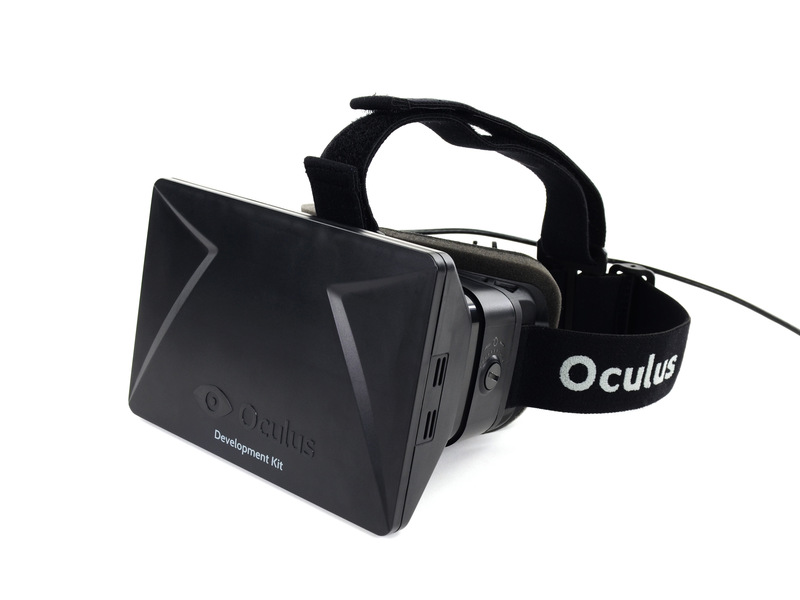
\includegraphics[width=0.3\textwidth]{dk1.jpg}
		    \caption{L'Oculus Rift (DK1)}
		  \end{figure}
		  \FloatBarrier
		  \subsubsection{Fonctionnement}
		  
			\paragraph{Matériel} ~\\
		    
				L'Oculus Rift est composé de:\\
			      
				\begin{itemize}
				\item Un écran 60 Hz d'une résolution de $1280*800$
				\item Deux lentilles (une pour chaque oeil),
				\item Un gyroscope à 3 axes pour mesurer l'accélération angulaire,
				\item Un magnétomètre à 3 axes pour mesurer les champs magnétiques,
				\item Un accéloromètre à 3 axes pour mesurer l'accélération, y compris gravitationnelle
				\item Un port USB
				\item Un port HDMI
				\end{itemize} ~
			      
				Il est à noter que la résolution de l'écran est à diviser par deux, chaque oeil voyant seulement
				une moitié de l'écran, la résolution effective est donc de $640*800$.
		    
			\paragraph{Logiciel} ~\\
			  
			    L'utilisation de l'Oculus Rift s'effectue au moyen de son SDK, qui permet:\\
			    
			    \begin{itemize}
			    \item D'accéder aux différents capteurs,
			    \item D'accéder aux propriétés du masque (distance inter-pupillaire, hauteur des yeux, \ldots),
			    \item D'appliquer les <<filtres>> au rendu graphique afin d'avoir un rendu réaliste
			    \end{itemize} ~
			    
			    Le SDK est écrit en C++ et possède une API en C.
			    Pour mon stage, j'ai utilisé la version 2.5 puis la version 0.3.2.
			
			\paragraph{Théorie} ~\\
			
			    L'Oculus Rift exige que la scène soit rendue graphiquement en <<split-screen stereo>>, 
			    c'est-à-dire avec l'écran divisé en deux verticalement, la partie gauche réservée à l'oeil gauche
			    et la partie droite à l'oeil droit.
			    
			    La distance inter-pupillaire est la distance entre les deux yeux. Elle varie d'un individu
			    à l'autre mais elle est en moyenne de 65 mm. Cette distance est importante dans le procédé 
			    de rendu car ce dernier consiste à rendre graphiquement la scène deux fois, une fois pour
			    chaque oeil, en translatant la caméra de la distance inter-pupillaire entre les deux rendus.
			    C'est ce qui contribue à créer l'effet stéréoscopique, ce qui engendre l'impression d'immersion.
			
			    Un autre aspect à prendre en compte est la présence des lentilles. Ces dernières agrandissent
			    l'image pour fournir un champ de vision très large, pour améliorer l'immersion.
			    Cependant ce procédé déforme l'image de façon significative, ce qui créerait une distortion
			    en coussinets si les <<filtres>>, dont nous parleront plus tard,
			    n'étaient pas appliqués au niveau logiciel au rendu graphique de l'application.\\
			    \FloatBarrier
			    \begin{figure}[h!]
			      \centering
				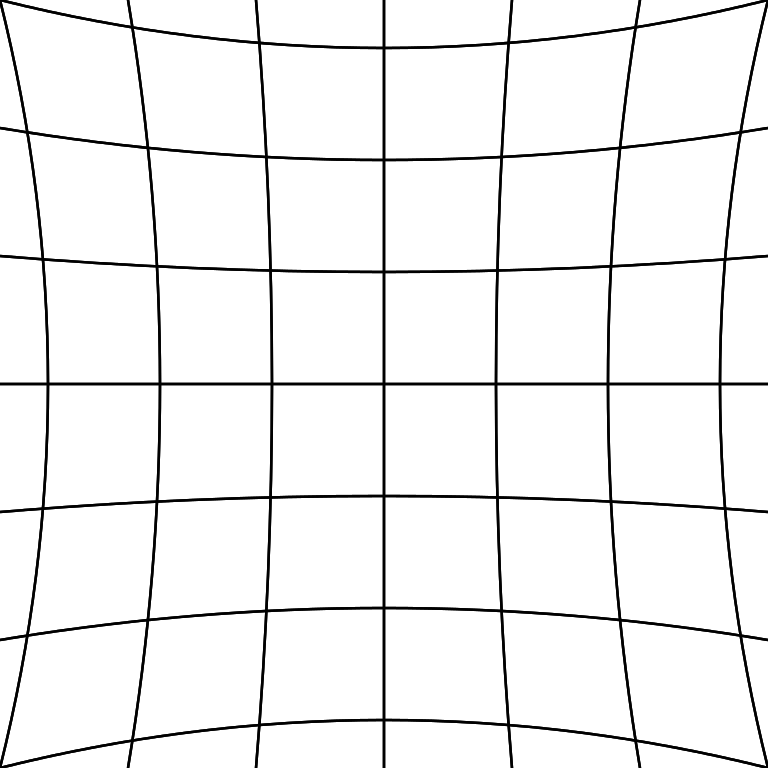
\includegraphics[width=3cm]{pincushion_distortion.png}
			      \caption{Distortion en coussinets (<<pincushion distortion>>)}\par\medskip
			    
			    \FloatBarrier
			    Pour contrebalancer cette distortion, le programme doit, comme énoncé plus haut, appliquer
			    un effet post-rendu. Il s'agit d'une distortion égale et opposée, appelée distortion en 
			    barillets.\par\bigskip
			    
			    {
			      \centering
				
\includegraphics[width=3cm]{barrel_distortion.png}
			      \caption{Distortion en barillets (<<barrel distortion>>)}
			    }\par\medskip
			    \FloatBarrier
			    De plus, le programme doit corriger les aberrations chromatiques, qui consistent en un effet
			    d'arc en ciel aux contours des objets. Cet effet est causé par les lentilles et est
			    bien connu dans le domaine de l'optique.\par\bigskip
			    \FloatBarrier
			  {
			      \centering
				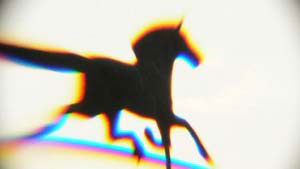
\includegraphics[width=4cm]{chromatic_aberration.jpg}
			      \caption{Aberration chromatique (<<chromatic abberration>>)}
			  }
			    \end{figure}  ~ \\
			    
			    \FloatBarrier
			\paragraph{Pratique} ~\\
			
			    Pour le développeur, ces éléments théoriques sont gérés de manière interne par le SDK Oculus.
			    
			    Pour une application qui fait un rendu graphique, la programme est typiquement de
			    la forme:\\
			    
			    \label{mainloop_normal}
			    \begin{algorithm}[H]
			      initialize the graphic ressources\;
			      fill the scene with graphic objects\;
			      \While{the application is running}{
				process the user input\;
				update the objects in the scene\;
				render the objects in the scene\;
			      }
			      release the graphic ressources\;
			      \caption{Application de rendu graphique}
			    \end{algorithm} ~\\
			    
			    Un programme qui fait un rendu Oculus exclusivement aura pour sa part la forme suivante:\\
			    \label{mainloop_oculus}
			    \begin{algorithm}[H]
			      initialize the graphic ressources\;
			      initialize the Oculus SDK\;
			      fill the scene with graphic objects\;
			      \While{the application is running}{
				process the Oculus input\;
				update the objects in the scene\;
				\For{each eye}{
				  translate the camera by the inter-pupillary distance\;
				  apply the Oculus distortion effects\;
				  render the objects in the scene\;
				  }
			      }
			      release the Oculus SDK\;
			      release the graphic ressources\;
			      \caption{Application de rendu graphique}
			    \end{algorithm} ~\\
			    Plus précisément, l'opération <<apply the Oculus distortion effects>> se fait de façon graphique
			    au moyen de shaders, qui sont des programmes qui appliquent des transformations à chaque pixel de l'image.
			    

			    Nous avons alors le rendu suivant, pour une scène simple composée d'un cube texturé, d'un plan
			    et d'une skybox rudimentaire, avec le même point de vue:
			    
			    \FloatBarrier
			    
			    \begin{figure}
			      \centering
				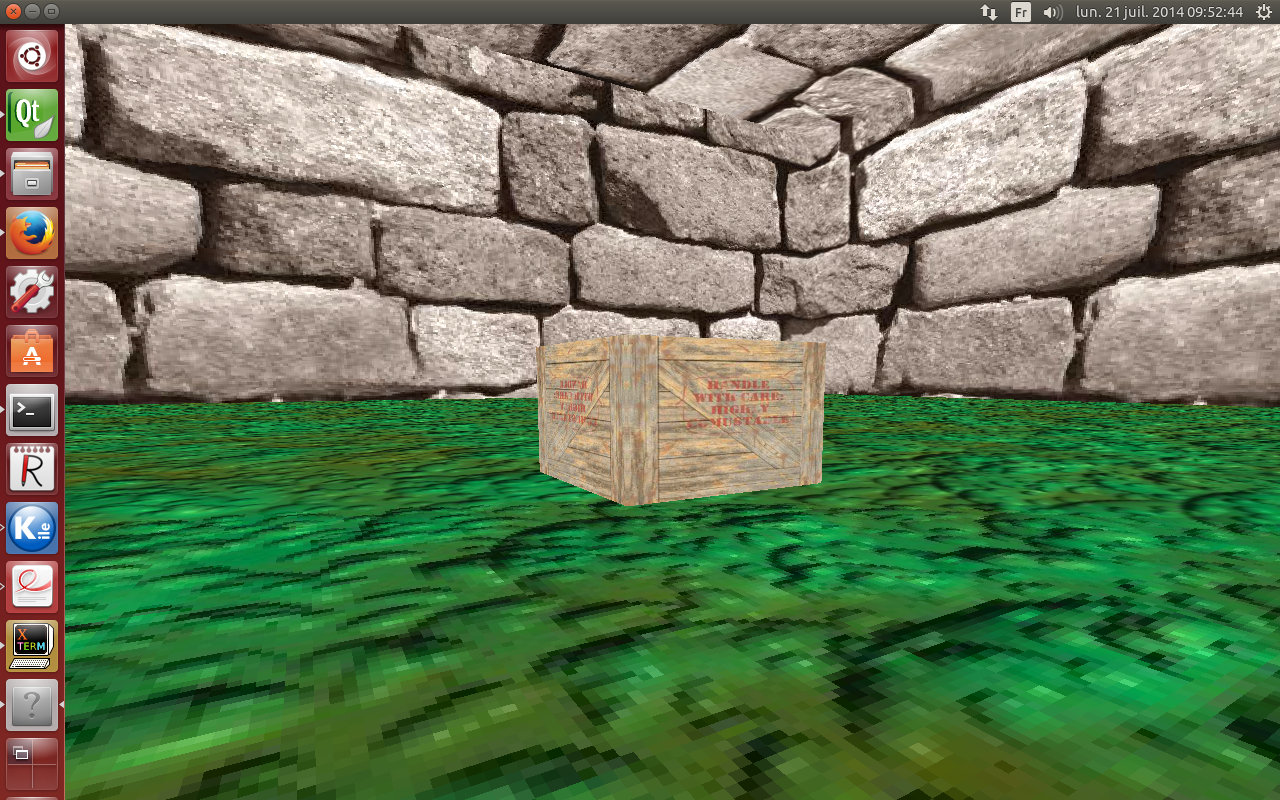
\includegraphics[width=1.0\textwidth]{scene_normal4.png}
			      \caption{Scène OpenGL simple avec le rendu normal}

				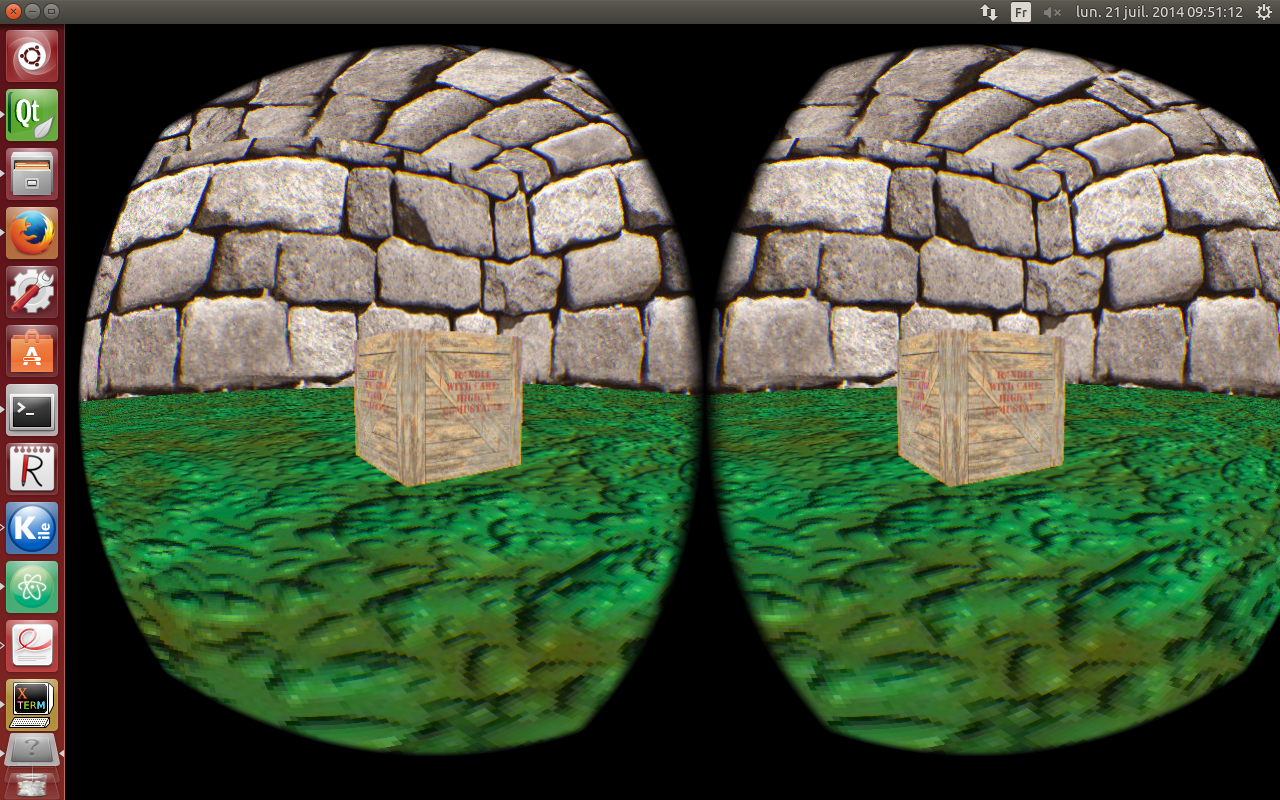
\includegraphics[width=1.0\textwidth]{scene_oculus4.png}
			      \caption{Scène OpenGL simple avec le rendu Oculus}
			    \end{figure}
			    \clearpage
			    
			    \FloatBarrier
			    
			    Les applications que j'ai développées au sein de mon stage peuvent fournir le rendu normal 
			    et le rendu Oculus, selon l'option spécifiée.

		
	\subsection{Contraintes}
	
	\subsubsection{Skybot 3D}
	    \paragraph{Existant} ~\\
	    
		La contrainte principale pour le projet Skybot 3D a été de travailler avec du code existant non documenté,
		de taille conséquente (3840 fichiers, 22863 lignes de code).
		En effet, j'ai eu accès à une version de développement non finalisée et non encore publiée. Cependant j'ai 
		eu de riches échanges avec les développeurs par mail et vidéoconférence, et j'ai eu la chance
		de les rencontrer à la fin du stage.
		
	    \paragraph{Langages} ~\\
	      
		Une contrainte supplémentaire a été le conflit de langages: le programme existant est écrit en C, et le
		SDK Oculus en C++, exigeant en conséquence un compilateur C++. 
		C et C++ sont des langages proches de par leur origine et leur histoire, C++ étant issu de C, 
		ils sont donc en grande partie compatibles. La majorité du code n'a donc pas posé de problème, 
		mais certains motifs ont dû être modifiés, notamment les conversions de types implicites,
		les arithmétiques de pointeurs et les pointeurs de fonctions ont du être réécrits de manière
		idiomatique en C++.
		
	    \paragraph{Versions d'OpenGL} ~\\
	    
		Une contrainte additionnelle, et peut-être la plus importante, a été l'utilisation de différentes 
		fonctionnalités d'OpenGL, appartenant à des versions différentes.
		En effet, la totalité du rendu graphique dans l'application existante se fait avec le <<fixed pipeline>> 
		d'OpenGL, c'est-à dire une suite d'opérations fixes de rendu. Cela consiste a faire un rendu graphique basé sur des
		appels à des fonctions OpenGL qui fournissent des fonctionnalités bien pratiques, comme des transformations
		matricielles, des lumières, \ldots Cependant ces appels, typiques d'OpenGL 1.x et 2.x, 
		utilisent principalement le CPU et ont donc
		été dépréciés pour des raisons de performances dans OpenGL 3.x et 4.x, au profit d'une programmation
		<<tout shader>>. Les shaders sont des programmes appliquant des effets sur chaque pixel de l'image et qui
		sont exécutés sur la carte graphique.
		
		Le développeur doit donc maintenant tout faire manuellement mais cela au profit des performances et de l'éventail
		de possibilités, mais au détriment de la simplicité.
		
		Le SDK Oculus utilise les shaders pour appliquer les effets graphiques mentionnés plus tôt (distortion, 
		correction des aberrations, \ldots), et cela a créé quelques conflits au niveau du rendu graphique, 
		avec le rendu existant n'utilisant pas ces shaders.
		
	    \paragraph{Échelles} ~\\
	      Skybot 3D est une simulation du système solaire et en tant que telle manipule des distances très grandes.
	      Cela n'est pas gênant sauf lorsque deux distances très grandes sont multipliées entre elles, par exemple
	      dans un calcul matriciel.
	      Cela peut provoquer un <<overflow>> (<<dépassement>>), phénomène consistant en une variable ayant une valeur
	      plus grande que ce que son type peut stocker en mémoire. Dans le meilleur des cas cela occasionne des 
	      erreurs d'arrondis causant des tremblements de la caméra ou des objets, des effets de <<flashing>> et
	      <<tearing>> dans le rendu, et dans le pire des cas un crash du programme.
	      
	      Dans mon cas, ce phénomène a provoqué un phénomène de <<cross-eye>> gênant pour l'utilisateur en mode
	      Oculus (\ref{cross_eye}).
		
	    \subsubsection{Simulation}
		\paragraph{Portabilité} ~\\
		  \epigraph{I don’t care if it works on your machine!  We are not shipping your machine!}{Vidiu Platon}
		
		  Pour ce projet, il a été convenu dès le départ d'assurer la portabilité du programme, c'est-à-dire
		  le fonctionnement multiplateforme.
		  
		  Dans cette optique, j'ai choisi un langage fonctionnant sur n'importe quelle plateforme existante 
		  (dès lors qu'il existe un compilateur adéquat), le C++, et
		  des bibliothèques multiplateformes, notamment pour le rendu graphique,
		  pour permettre l'abstraction d'une API spécifique à une plateforme donnée, en fournissant une API générique.
		  Un exemple est l'utilisation de la SDL, une bibliothèque de fenêtrage, ou d'OpenGL, une API de rendu
		  graphique.
		  
		  De plus, un soin particulier a été porté dans le développement à  l'évitement de l'introduction 
		  de code spécifique à une plateforme donnée. Une solution a été l'utilisation maximale de la libraire 
		  standard du langage.
		  
		  Enfin j'ai utilisé un outil de compilation multi-plateforme, qmake, qui permet de compiler le code
		  sur plusieurs plateformes différentes automatiquement.
		  
		  Au final, j'ai uniquement travaillé sur Linux mais le code fonctionne selon toute probabilité sur 
		  Windows et OSX, avec des drivers à jour, sur des versions relativement récentes de ces systèmes d'exploitation.
		  
		\paragraph{Taille des données} ~\\
		
		  Comme évoqué plus haut, j'ai travaillé sur des données avoisinant le million d'objets. Cela a posé
		  principalement un problème de performances. En effet, c'est en travaillant avec de tels nombres que
		  l'on se rend compte de la disparité CPU (processeur) / GPU (carte graphique).
		  En effet, malgré un processeur avec 16 GB de RAM, le fait de parcourir tous les objets pour les afficher (une fois par frame, $\mathcal{O}(n)$),
		  prenait plus de 16 millisecondes, nombre critique dans le domaine du rendu graphique, puisqu'il
		  correspond au temps de rendu maximal d'une frame si l'on veut un rendu à 60 FPS (frame per seconds),
		  ce qui fournit une expérience correcte pour l'utilisateur: $1000 ms / 60 = 16.666 ms$.
		  
		  En sus, comme j'ai travaillé avec cubes de données (corps célestes dont les cooordonnées spatiales se trouvent toutes
		  contenues dans un cube, typiquement de taille 64*64*64 ou 100*100*100), ce qui peut donner une boucle de rendu
		  de complexité $\mathcal{O}(n^3)$, empirant alors le temps de rendu.
		  
		  De plus, il faut garder à l'esprit que l'objectif final est d'avoir un rendu Oculus valide. Or le
		  SDK Oculus fait un double rendu (un pour chaque oeil), en appliquant des transformations matricielles
		  pour chacun des rendus. Il est donc primordial d'avoir des FPS corrects dans le rendu graphique normal.
		  
		  Cependant, je me suis aperçu que la carte graphique ne rencontrait pas de problème de temps de rendu,
		  gardant la plupart du temps un temps de rendu d'une frame inférieur à la milliseconde.
		  
		  Dès lors, plusieurs solutions se sont présentées:
		  
		  \begin{description}
		  \item [Travailler avec un seul objet graphique]~\\ Cela consiste à avoir un seul objet dans le programme qui 
		  contient les coordonnées de tous les objets célestes. On <<boucle>> donc sur un seul objet et on envoie toute
		  les positions des objets célestes en une seule fois comme s'il n'y avait q'un objet et la carte
		  graphique fait tout le travail. Cela fonctionne mais est peu flexible (comment faire pour sélectionner
		  un seul objet céleste pour afficher des informations à son sujet?) et on atteint les limites de la
		  carte graphique pour un très grand nombre d'objets. Cependant le CPU a un minimum de travail.
		  
		  \item [Octree]~\\ Un Octree est un arbre où chaque noeud (appelé <<octant>>) compte jusqu'à 8 fils. Il correspond à partition
		  d'un espace cubique, à la manière d'un quadtree en 2D, et permet de diviser notre scène en régions,
		  contenant elles-mêmes des sous-régions et ainsi de suite. On peut alors décider d'afficher seulement les
		  régions voisines de notre position sans afficher les régions que l'on ne peut pas voir ou qui sont
		  trop lointaines. C'est la solution que j'ai choisie car c'est la plus flexible et celle qui offre le
		  plus de possibilités. A noter cependant que cela impose une taille de cube d'une puissance de deux.
		  \FloatBarrier
		  \begin{figure}
			      \centering
				\includegraphics[width=0.5\textwidth]{octree.png}
			      \caption{Schématisation d'un octree}
			      
		   \end{figure} 
		    
		
			      
		\begin{figure} 
			\centering
				\includegraphics[width=0.4\textwidth]{octree2.jpg}
			      \caption{Octree en action}
		  
		\end{figure}
		  \FloatBarrier
		\end{description}

		  
		On optimise alors le rendu à la fois sur le CPU (moins d'objets parcourus dans la boucle
			      de rendu à chaque frame) et sur le GPU (moins de données envoyées et 
			      rendues graphiquement à chaque frame).  
				
		
		Initialement, mes objets étaient tous stockés dans un tableau que je parcourais à chaque frame pour les afficher.
		Pour 1000 objets, j'avais une moyenne de 5 FPS. 
		J'ai alors mis en place un Octree. J'ai eu alors des FPS variant entre 30 et 60 FPS, avec une moyenne de 55 FPS
		(le rendu est limité à 60 FPS maximum
		pour ne pas surcharger le CPU/GPU), quelque soit le nombre d'objets présents dans la scène, ce qui est acceptable.
		En effet, l'Octree permet d'afficher un nombre moyen constant d'objets quelque soit notre position.
		Avec un cube de taille 128*128*128 et 32768 objets, le temps de génération de l'Octree est d'environ 120s.
		J'affiche l'octant (et donc tous les objets célestes se trouvant dans cet octant) où la caméra se trouve
		et les 6 octants immédiatement voisins, avec une taille d'octant de 8.
		Pour résumer, on sacrifie le temps de démarrage du programme au profit des performances à l'exécution.


	
		
	\subsection{Déroulement du stage}
	
	   \epigraph{Premature optimization is the source of all evil}{Donald Knuth}
	   
		Mon stage s'est principalement déroulé en trois temps: formation, développement, optimisation.
		
		La première semaine a été consacrée à la découverte de l'Oculus Rift, l'essai de démos, et l'installation
		des outils de développement.
		
		La deuxième et troisième semaine ont consisté à se former à l'Oculus SDK et OpenGL, et à tester la
		faisabilité de l'intégration de l'Oculus Rift à un moteur de rendu 3D existant, Irrlicht. Malheureusement 
		cela s'est révélé plus complexe que prévu et la décision a été prise d'utiliser OpenGL sans framework,
		vu le temps imparti.
		Cette période a aussi servi à se (re)former au C++. C'est un langage que j'avais déjà utilisé sur d'anciens
		projets mais les nouveautés introduites par C++11 m'étaient inconnues.
		
		La quatrième et cinquième semaine ont été centrées sur le développement de programmes minimalistes mettant
		en place OpenGL et l'intégration de l'Oculus Rift, et la découverte du code source de Skybot 3D.
		
		La sixième, septième et huitième semaine ont été axées sur le développement de mes deux projets.
		
		La neuvième et dixième semaine ont porté sur la rédaction de ce rapport et sur les possibles optimisations
		des deux projets, ainsi que la refactorisation du code et la documentation complète.
				
		Je me suis toutefois formé tout au long de mon stage à OpenGL, notamment à propos
		des différences entre les versions 1.x/2.x et 3.x/4.x, où la philosophie du <<tout shader>> a été introduite,
		et la compatibilité entre ces versions.
		
		
	
	\subsection{Développement}
	
	  \subsubsection{Bonnes pratiques}
	    \epigraph{Always code as if the guy who ends up maintaining your code will be a violent psychopath who knows where you live}{Martin Golding}
	    \epigraph{Programs must be written for people to read, and only incidentally for machines to execute}{Arold Abelson}
	    
	    Comme mentionné plus tôt, j'ai tout au long de mon stage versionné mon code avec git et Github, ce qui a
	    permis de le partager facilement avec l'équipe Skybot 3D et André SCHAAF.
	    
	    De plus j'ai régulièrement utilisé des outils d'analyse statique et dynamique pour jauger de la qualité de
	    mon code et l'améliorer.
	    
	    En sus, j'ai activé les options de compilation aidant dans cette tâche: <<-Wall>>, <<-Wextra>>, <<-Werror>>, \ldots
	    
	    
	    
	    J'ai également entièrement documenté mon code avec l'outil dédié Doxygen, et gardé une constance dans le nommage des variables,
	    l'indentation du code, \ldots
	    
	    Enfin, j'ai utilisé deux compilateurs différents, clang et gcc, en comparant leurs performances,
	    notamment avec les options d'optimisations <<-O1>>, <<-O2>>, <<-O3>>, <<-Ofast>>.
	    Pour finir, j'ai utilisé le déboggeur gdb et l'analyseur de mémoire Valgrind pour vérifier que mon application
	    était exempte de fuites mémoires (mis à part celles provenant du SDK Oculus pour lesquelles je ne peux rien faire).
	    
	    
	  \subsubsection{Design Patterns}
	      \epigraph{Controlling complexity is the essence of computer programming}{Brian Kernighan}
	      
	      
	      
	    Les design patterns sont des motifs de programmation, des <<façons de faire>> que l'on retrouve régulièrement 
	    pour résoudre des problèmes bien connus. Ce ne sont pas des <<tours de magie>> ou des  <<gadgets à la mode>>,
	    mais des solutions pratiques à mettre en place quand le besoin s'en fait sentir, ou pour améliorer le code.
	    
	    Pendant ce stage, j'ai utilisé plusieurs design patterns. Voici lesquels et pourquoi:
	    
	    \begin{description}
	    \item [NullObject pattern]~\\
		Ce design pattern sert à gérer élégamment la situation où l'on a un ensemble d'objets à gérer dont certains sont
		nuls, sans savoir lesquels à l'avance, ou sans vouloir vérifier à chaque utilisation. Plutôt que d'écrire des dizaine de conditions pour vérifier si l'on peut bien effectuer telle ou telle action
		afin d'éviter une segmentation fault, la variable sur laquelle nous sommes en train de travailler
		étant nulle (c'est-à-dire ayant pour valeur le pointeur <<NULL>> ou <<nullptr>> en C++11),
		ce pattern propose de travailler avec une classe générique. De cette dernière hérite(nt) la ou les classe(s) dont nous nous
		servons en pratique dans notre programme, et une classe <<NullObject>> dont le corps des méthodes sont vides (ou
		adaptées selon la situation).
		Ainsi au lieu de travailler avec des pointeurs nuls, on travaille avec de vrais objets, inoffensifs lorsque
		l'on intéragit avec eux, grâce au polymorphisme.
		Ce faisant on peut aussi élégamment activer/désactiver des services.\\
		
		Dans mon cas, j'ai travaillé avec la classe <<GraphicObject>>, dont héritent les classes <<Cube>>, <<Plane>>, \ldots,
		mais aussi <<NullGraphicObject>>, dont la méthode d'affichage ne faisait rien.
		Ainsi dans ma boucle de rendu, je pouvais afficher tous mes objets de la scène, sans avoir peur que certaines parties
		de l'Octree soient vides et que cela occasionne un plantage.
		
		
		De la même façon, j'ai utilisé ce pattern pour gérer les deux modes de rendu. J'ai une classe <<GenericOculus>>,
		dont héritent les classes <<NullOculus>>, dont les méthodes sont vides, et <<Oculus>>, où est implémenté
		le rendu Oculus. Dans le mode normal, j'utilise la classe <<NullOculus>> qui ne fait rien, tandis qu'en mode
		Oculus j'utilise la classe <<Oculus>>.

	    \item [Singleton pattern]~\\
		Design pattern bien connu et parfois décrié, il permet de limiter le nombre d'instances d'un objet, typiquement
		à 1.\\
		
		Je l'ai utilisé pour la classe Oculus, afin d'éviter de faire l'initialisation (et la libération) du SDK Oculus plusieurs fois.
		
	    \item [Game Loop pattern]~\\
		Ce pattern décrit la boucle de rendu typique d'une application de rendu graphique.
		
		Je l'ai utilisé pour l'application de simulation, comme décrit ici~(\ref{mainloop_normal}) pour le rendu normal
		et là~(\ref{mainloop_oculus}) pour le rendu Oculus.
	    
	    \item [Flyweight Pattern]~\\
	      Ce pattern sert à améliorer les performances d'une application où sont présents de nombreux objets identiques,
	      mis à part la valeur de certaines propriétés, et qui utilisent des ressources similaires.
	      Au lieu que chaque objet possède une instance de la ressource, générant une perte de performances
	      inutile, ce pattern propose de mettre en commun tout ce qui peut l'être. Chaque objet aura alors un pointeur
	      vers la ressource partagée. Ce partage est transparent pour l'application qui continue à utiliser les objets 
	      comme bon lui semble, en utilisant les informations particulières de chaque objet.\\
	      
	      Dans ma situation, la simulation concerne des milliers voire des millions d'objets célestes. Dans les cas que j'ai
	      rencontrés, il s'agissait toujours d'un seul type d'objet céleste, par exemple une étoile.
	      Si l'on choisit de représenter une étoile par un modèle 3D, une sphère par exemple, et une
	      texture plaquée sur cette sphère, et que l'on charge la ressource <<texture>> à partir d'un fichier, il est inconcevable
	      de lire ce fichier des millions de fois par seconde (à chaque rendu), ou même des millions de fois au démarrage du
	      programme (initialisation des textures des objets célestes).
	      On choisit alors de charger cette ressource une fois pour toute au démarrage. On lit une et une seule fois le fichier.
	      Chaque étoile possède un pointeur vers cette texture partagée. 
	      La seule différence entre les étoiles sont les informations contextuelles (position, densité, âge, \ldots).
	      
	      On peut alors faire le rendu sans problème de performances: au final, on fait une seule lecture de fichier, et
	      l'on a une seule texture en mémoire, au lieu de milliers/millions auparavant.
	      L'initialisation prend ainsi moins de temps et la libération mémoire également à la fin du programme.
	      
	      En pratique, l'application de ce design pattern a permis de transformer un démarrage poussif (dizaines de secondes) avec 100 objets célestes,
	      en un démarrage en environ 3s pour 1000 objets.
	    
	    \item [Factory pattern]~\\
	      Ce pattern permet typiquement de créer dynamiquement des instances d'objets différents, dont le type 
	      n'est connu qu'à l'exécution (par exemple conséquence d'un choix utilisateur).
	      Cependant il peut aussi être utilisé pour encapsuler la construction d'un objet derrière une interface
	      qui fait des vérifications diverses à cette occasion.
	      
	      Dans mon cas, je l'ai utilisé pour implémenter le groupe de textures partagées. En effet lorsqu'un nouvel
	      objet graphique texturé est créé, il fait une requête auprès de la fabrique de textures pour obtenir sa texture.
	      La fabrique vérifie si la texture existe déjà en mémoire.
	      Si oui elle renvoie un pointeur vers cette texture, sinon elle créé la texture correspondante, l'ajoute 
	      au groupe de textures partagées, et finalement renvoie un pointeur vers cette texture nouvellement créée.
	      
	      L'avantage d'avoir une fabrique de textures est que cette dernière peut être utilisée par plusieurs classes
	      différentes: dans mon cas la classe <<Crate>> (<<caisse>>, qui représente un cube texturé) et <<Plane>>, 
	      (<<plan>>, qui représente un surface plane texturée) utilisent le groupe de textures partagées, et donc 
	      font appel à la fabrique.
	      Ainsi cette logique n'est pas inhérente à une classe et peut être utilisée partout dans le programme.
	      De plus si deux classes différentes utilisent la même texture, une seule sera créée, et non deux.
	    
	    \item [RAII]~\\
	      \label{RAII}
	      <<Resource Acquisition Is Initialization>>, l'acquisition de ressources c'est leur initialisation.
	      Ce pattern permet une gestion efficace et simple de la mémoire et est inhérent au C++.
	      
	      Il repose sur l'assurance fournie par le langage que le destructeur d'un objet sera appelé lorsque l'on
	      sort du bloc où il a été défini.
	      Ainsi, lorsque l'on acquiert une ressource, par exemple ouvrir un fichier, et que cette ressource a besoin
	      d'être libérée plus tard, par exemple fermer ce fichier, on peut automatiser ces deux actions en les plaçant
	      à un endroit adéquat du code.
	      
	      En pratique, on fait l'acquisition dans le constructeur de l'objet utilisant/représentant la ressource (d'où le nom), et 
	      la libération dans le destructeur. Pour l'utilisateur de la classe ces opérations sont transparentes et il est
	      assuré qu'elles seront exécutées automatiquement.
	      
	      
	      Pour ma part, j'ai utilisé ce pattern pour l'initialisation et la libération des ressources graphiques et
	      du SDK Oculus.
	    
	    \item [Data Locality]~\\
	      Ce design pattern est un moyen d'optimiser les performances d'un programme en tirant parti du cache du CPU.
	      
	      En effet tous les CPU modernes disposent d'une certaine quantité de mémoire vive, la RAM, qui représentent
	      plusieurs Gigaoctets. Pour accélérer l'accès à cette mémoire, le CPU dispose d'un cache (plusieurs en réalité)
	      de taille réduite (sur ma machine je dispose d'un Intel Core i5 cadencé à 3.2 GHz avec 4 coeurs et 6144 kB
	      de cache), qui est en fait une zone mémoire à accès très rapide où sont stockées les informations dont l'accès est fréquent
	      dans la RAM. On accélère ainsi les opérations les plus régulièrement effectuées: c'est la mise en cache (<<caching>>).
	      
	      Cependant, le polymorphisme impose en C++ l'usage de pointeurs (cas le plus fréquent) ou de références (cas particuliers. 
	      Mais les pointeurs, par définition, pointent vers différentes zones mémoires.
	      Ainsi, lorsque l'on veut afficher tous les objets de la scène, on parcoure la structure de données qui
	      stocke les pointeurs sur tous ces objets et on les affiche un par un.
	      
	      Le problème est que contrairement au parcours d'un tableau de valeurs (non pointeurs), qui sont stockées
	      contigument dans la mémoire, et sont donc particulièrement adaptées à la mise en cache, le fait de
	      parcourir un tableau de pointeurs va silloner toute la RAM, et donc ne va pas du tout se prêter à la mise
	      en cache. Le CPU va soit ne pas mettre ces variables (et les zones mémoires voisines) dans le cache, soit le faire
	      et en conséquence changer la majeure partie du cache à chaque fois, ce qui n'est pas du tout optimal.
	      On passe donc à côté d'un beau gain de performance: c'est le <<cache miss>>.
	      
	      Plus généralement, cette situation se produit dès lors qu'il y a un usage fréquent de pointeurs dans un 
	      programme, et surtout le déréférencement de ces derniers.
	      
	      Un autre point à considérer est la différence entre l'utilisation , dans une structure de donnée, du polymorphisme (plusieurs objets
	      différents coexistent, héritant d'un objet commun) et l'utilisation d'un seul type d'objets.
	      Dans le second cas, une méthode appelé par un objet est déterminée à la compilation (on sait quel est le type
	      de l'objet puisqu'il n'y en a qu'un) tandis que dans le premier cas, elle est déterminée à l'exécution,
	      ce qui peut engendrer une baisse de performances supplémentaires.
	      
	      Pour résumer, le polymorphisme apporte généricité et flexibilité, mais peut engendrer une baisse de 
	      performances, alors que l'usage d'un seul type d'objets est plus rigide, mais peut améliorer les performances.
	      
	      Un dernier point à envisager est la différence de stockage des variables entre l'utilisation de pointeurs sur variables
	      et l'utilisation de variables. Dans le premier cas, les variables sont allouées (et libérées) manuellement et sont placées sur
	      le tas (<<heap>>), alors que dans le second cas elles sont allouées automatiquement sur la pile (<<stack>>).
	      Ces deux zones mémoires sont présentes dans chaque programme et sont réservées par le système d'exploitation
	      pour le programme à son lancement et sont fort différentes:\\
	      
	      Stack:
	      \begin{itemize}
		\item Accès rapide
		\item Limitée en taille
		\item L'espace est géré automatiquement et efficacement par le CPU (pas de fragmentation)
	      \end{itemize}~
	      
	      Heap:
	      \begin{itemize}
		\item Accès plus lent
		\item Pas de limite de taille
		\item Pas de gestion automatique de l'espace (fragmentation)
	      \end{itemize}~
	      
	      La fragmentation est l'utilisation inefficace de l'espace mémoire. C'est un phénomène qui se produit lorsque 
	      sont effectuées de multiples allocations et
	      désallocations de mémoire, engendrant alors une baisse de la capacité mémoire et/ou des performances.
	      
	      Ces allocations/désallocations ne sont pas non plus gratuites en termes de temps d'exécution, puisque
	      elles font appel à un certain nombre de fonctions.


	      Dans mon cas, j'ai donc transformé mon tableau de pointeurs sur objets célestes en un tableau d'objets célestes.
	      Cela est rendu possible par le fait que je ne dispose que d'un seul type d'objet céleste dans ma simulation.
	      De plus l'usage de pointeurs dans mon programme est majoritaire dans la partie génération et rendu d'objets célestes
	      de part leur nombre.
	      Cependant il est à noter que dans le cas d'un nombre très grand d'objets (de l'ordre du million), il est possible de dépasser
	      la taille de la pile, créant alors un <<stack overflow>>.
	      
	      J'ai ensuite mesuré les temps d'exécution dans les deux implémentations, exposés ici: \ref{optimisations}
	      et en ait tiré des conclusions suprenantes.
	    
	    \end{description}
%“Any fool can write code that a computer can understand. Good programmers write code that humans can understand.”
%- Martin Fowler (author and speaker on software development)
	
	\subsubsection{Architecture}
	\epigraph{Perfection [in design] is achieved, not when there is nothing more to add, but when there is nothing left to take away}{Antoine de Saint-Exupéry}
	    \FloatBarrier
	    \begin{figure}
				  \centering
				  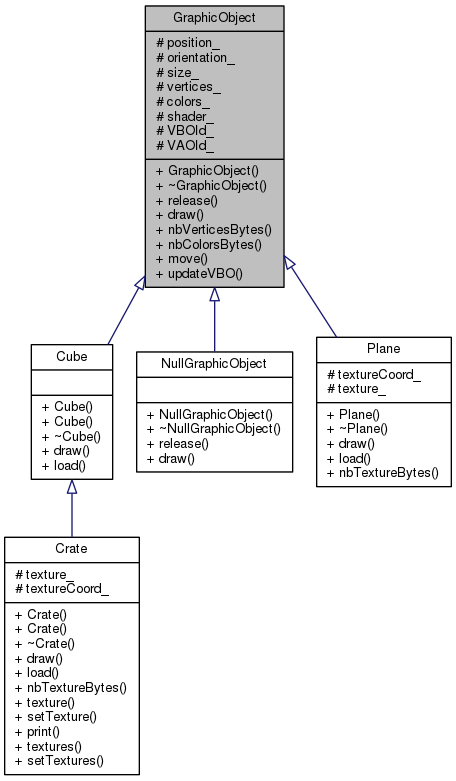
\includegraphics[width=0.8\textwidth]{uml1.png}
				  \caption{Diagramme de classe UML pour les objets graphiques}
	    \end{figure}
	    
	    \begin{figure}
			      \centering
			      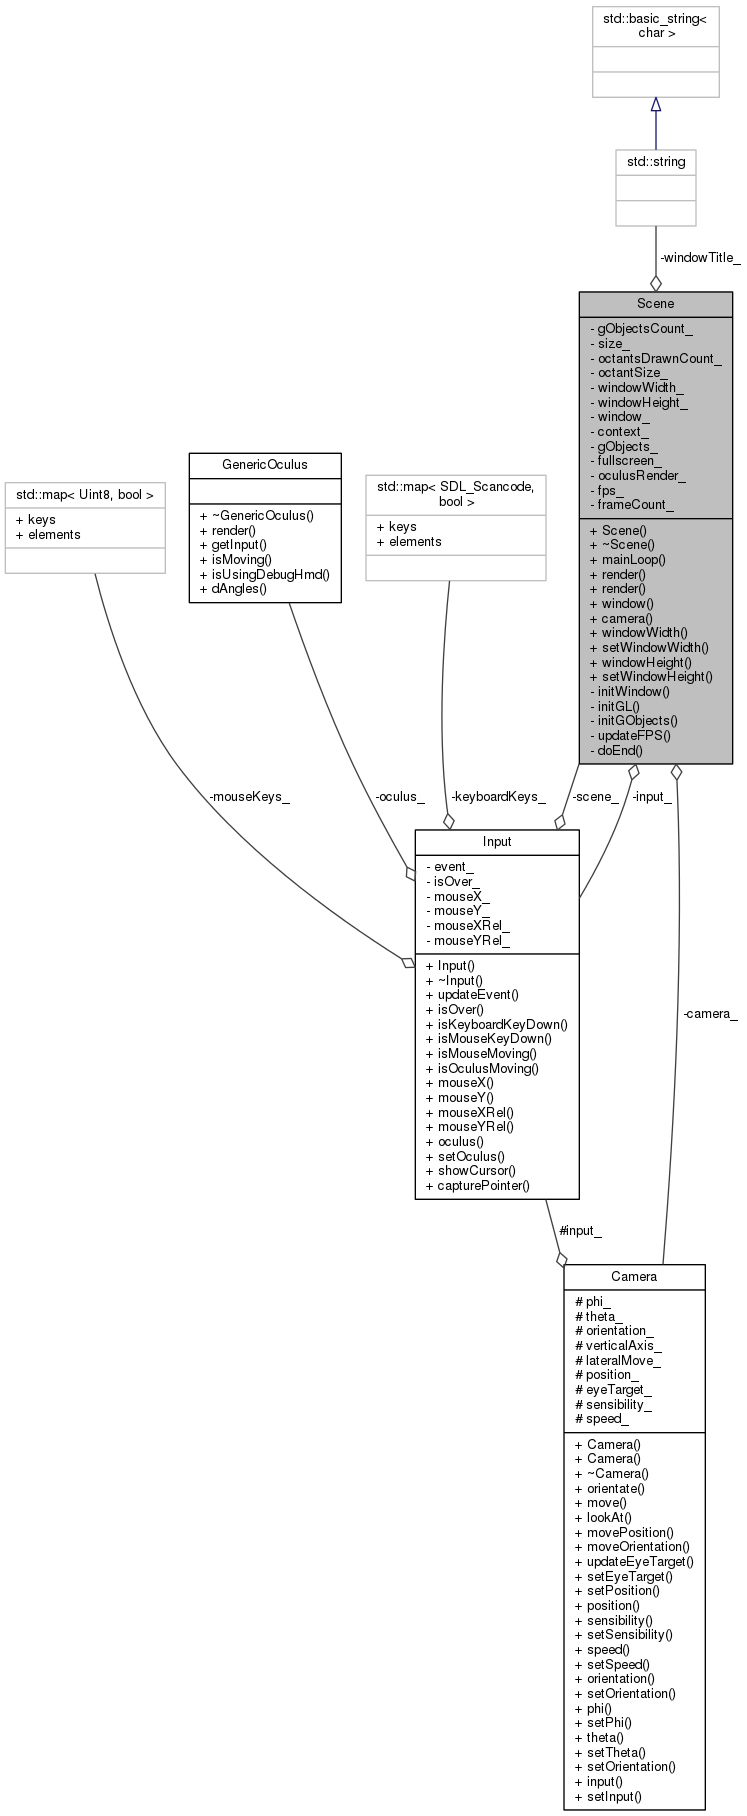
\includegraphics[width=0.6\textwidth]{uml2.png}
			      \caption{Diagramme de classe UML pour la scène}
	    \end{figure}
	    
	    \begin{figure}
			      \centering
			      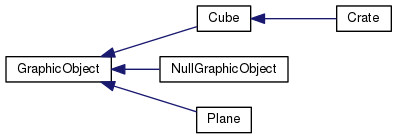
\includegraphics[width=0.8\textwidth]{hierarchy3.png}
			      \caption{Hiérarchie des classes}
	    \end{figure}
	    
	    \begin{figure}
	      \centering
	      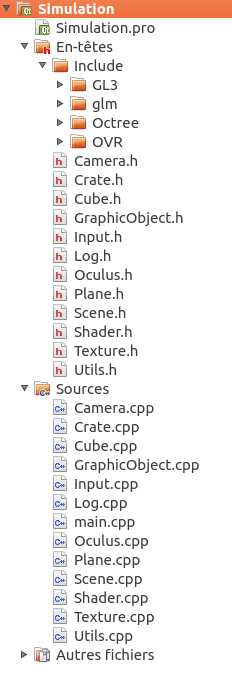
\includegraphics[width=0.3\textwidth]{files1.png}
	      \caption{Hiérarchie des fichiers}
	    \end{figure}
	    \FloatBarrier

  \subsection{Améliorations - Optimisations}
  
    \subsubsection{Structures de données - Data Locality}
    
      \begin{center}
      
	\label{optimisations}

	
	\begin{tabular}{| c | c | c | c | c | p{4cm} |}
	    \hline
	    Stockage & Méthode & Nombre d'objets & Génération & FPS moyens & Remarques \\ \hline
	    
	    Tableau & Polymorphisme & 1024 & 3.7 s & 37.2  & array\\ \hline
	    Tableau & Polymorphisme & 10000 & 38.2 s & 9.5  & array\\ \hline
	    
	    Tableau & Polymorphisme & 1024 & 3.6 s & 35.9  & vector, ajout avec push\_back \\ \hline
	    
	    Tableau & Polymorphisme & 10000 & 36.4 s & 9.6  & vector, ajout avec push\_back \\ \hline

	    
	    Tableau & Data locality & 1024 & 11 s & 35.6  & vector, ajout avec emplace\_back\\ \hline
	    Tableau & Data locality & 1024 & 11 s & 34.6  & vector, ajout avec push\_back\\ \hline
	    
	    
	    Tableau & Data locality & 1024 & 7.3 s & 34.2  & vector, ajout avec emplace\_back, réservation de la taille
								    requise à l'avance\\ \hline
	    Tableau & Data locality & 1024 & 7.2 s & 33.5  & vector, ajout avec push\_back, réservation de la taille
								    requise à l'avance \\ \hline
								    
								    
	    Tableau & Data locality & 10000 & 74.4 s & 9.2  & vector, ajout avec emplace\_back, réservation de la taille
								    requise à l'avance\\ \hline								    
	    Tableau & Data locality & 10000 & 71 s & 9.2  & vector, ajout avec push\_back, réservation de la taille
								    requise à l'avance\\ \hline	
								    
								    
	    Octree & Polymorphisme & 1024 & 3.6 s & 62.5 & \\ \hline
	    Octree & Polymorphisme & 32768 & 120 s & 62.5 & \\ \hline
	    
	    \hline
	\end{tabular}
      \end{center}
	
	La structure <<vector>> est un tableau dynamique de la librairie standard. 
	Sa méthode <<reserve>> permet de réserver une certaine taille à l'avance. Cela permet d'éviter, lors de l'ajout
	d'un nouvel objet, que la zone mémoire que le vector occupe se révèle trop petite, et qu'il faille en
	réallouer une nouvelle, en y déplaçant tous les éléments existants du vector. On voit que l'usage de cette méthode
	fait gagner quelques secondes pour la génération de 1024 objets (on passe de 11s à 7s).
	La structure <<array>> est un tableau statique de la librairie standard.
	
	On ne remarque cependant pas de différence majeure de performances entre ces deux structures de données une fois
	que la taille nécessaire en mémoire est réservée initialement.
	
	Un autre point à noter est la croissance linéaire du temps de génération en fonction du nombre d'objets, ce qui
	est prévisible étant donné que les structures de données array et vector sont de complexité linéaire pour le parcours
	et l'ajout.
	
	Cependant l'évolution du nombre de FPS en fonction du nombre d'objets n'est pas linéaire: cela est probablement
	dû au fonctionnement interne d'OpenGL.
	
	Les résultats de la comparaison entre usage du polymorphisme et usage du pattern Data Locality 
	sont surprenants: en effet, l'application de ce design pattern a ralenti les performances 
	de l'application, en tout cas dans la partie génération, le rendu graphique restant inchangé avec 
	      des FPS constants, au lieu de les améliorer.
	      
	      Cela s'explique par le fait que ce pattern améliore les performances d'applications ralenties par les 
	      <<cache misses>>. Lors de l'analyse de l'application par un outil d'analyse de cache, Valgrind, il est
	      apparu que seulement 0 à 2\% des accès au cache créaient des <<cache misses>>. Le problème de performances
	      n'était donc pas dû à cela.
	      
	      Pourquoi alors les performances ne sont-elles pas restées constantes? En fait, au lieu de stocker dans notre
	      structure de données un pointeur sur objet, qui prend typiquement 4 octets en mémoire, on stocke 
	      l'ensemble de l'objets, c'est à dire dans mon cas 136 octets. En C++, le passage d'un argument
	      à une fonction se fait par défaut par valeur, c'est à dire qu'il y a une copie de l'objet.
	      On copie donc 136 octets (au lieu de 4 auparavant) à chaque fois que l'on ajoute un objet dans la structure de données, et ce 
	      autant de fois qu'il y a d'objets. C'est ce qui ralentit la génération.
		      
	L'application du pattern Data Locality s'est donc révélé infructueux dans mon cas. Ce pattern reste cependant valide
	dans le cas d'applications souffrant de problèmes de <<caches misses>> et de fragmentation.
	
      \subsubsection{Smart pointers (<<Pointeurs intelligents)}
	\epigraph{You can either have software quality or you can have pointer arithmetic, but you cannot have both at the same time}{Bertrand Meyer}
	
  
	Les smart pointers sont des objets de la librairies standard encapsulant les pointeurs.
	En se basant sur la RAII (\ref{RAII}, paragraphe <<Design Pattern>>), ils permettent de s'assurer que les ressources mémoires allouées manuellement
	seront bien libérées.
	De plus ils fournissent des fonctionnalités bien pratiques, comme le compte de pointeurs pointant sur la variable encapsulée,
	 sorte de compte de références, pratique pour implémenter un groupe de ressources partagées: lorsque plus personne
	 dans le programme n'utilise ces ressources, on les supprime, ou plutôt elles sont supprimées automatiquement.
	 
	C'est ce qui s'approche en C++ d'un garbage collector, à la différence que la norme du langage assure
	à quel endroit du code le destructeur de l'objet sera appelé et que le développeur doit mettre en place manuellement
	cette gestion <<automatisée>>, ou plutôt <<aidée>>,  de la mémoire.
	 
	L'utilisation de ces pointeurs intelligents est considérée dans le monde du développement C++ comme une bonne 
	pratique et est encouragée. De plus il n'y a peu ou pas de baisse de performances par rapport à l'utilisation
	de pointeurs nus (<<raw pointers>>, pointeurs traditionnels <<à la C>>).
	
	Cette optimisation ne vise donc pas les performances mais la maintenabilité, la sécurité et la stabilité du programme.
	Au final, pour générer 1024 objets, la différence entre pointeurs nus et pointeurs intelligents est de 0.06 s,
	et il n'y a aucune fuite mémoire. De plus le code est plus court et plus simple.
	

      \subsubsection{Logs}
	\epigraph{There are two ways to write error-free programs; only the third one works}{Alan J. Perlis}
      
	Les logs sont l'affichage de messages de contrôle au cours du programme. Ils permettent de vérifier son exécution
	et de détecter des bugs.
	Après avoir utilisé des logs rudimentaires, je me suis intéressé aux bibliothèques de logs existantes, notamment Boost.Log .
	
	Cependant, ces bibliothèques se sont révelées bien trop riches et complexes pour la taille de ce programme.
	J'ai donc développé une classe simple de logs, qui offrent les fonctionnalités simples suivantes:
	
	\begin{itemize}
	 \item Quatre niveaux de logs différents (trace, debug, info, error),
	 \item Logs dans la console (activable/désactivable),
	 \item Logs dans des fichiers <<.log>> et <<.err>> selon le niveau du log (activable/désactivable),
	 \item Filtre des logs selon le niveau,
	 \item Syntaxe simple
	\end{itemize}~
	
	Cette amélioration n'est pas directement liée aux performances, mais vise à améliorer encore une fois la maintenabilité
	et la stabilité du code.
	Cependant, les performances de l'application bénéficient du fait que les logs soient désactivables en partie ou complètement, au choix.
	
    \subsubsection{Problèmes restants - Fonctionnalités à améliorer}
      \paragraph{Skybot 3D}~\\
	\label{cross_eye}
	Un problème handicapant restant dans Skybot 3D est la vue Oculus.
	En effet cette dernière est fonctionnelle, mais souffre du phénomène de <<cross-eye>> (<<yeux croisés>>).
	Cet effet est dû à une inversion du rendu entre les deux yeux: le rendu de l'oeil gauche se retrouve sur la moitié  droite sur
	l'écran et vice-versa.
	En conséquence, lorsque l'Oculus est équipé, les deux images provenant de chaque oeil ne se superposent pas
	parfaitement pour le cerveau comme cela devrait être le cas: une impression de strabisme (fait de loucher ) se produit.

	Malgré de nombreux efforts, ce phénomène est toujours en place et est probablement dû à une application erronnée
	des matrices de tranformation.
	
      \paragraph{Simulation}~\\
	Une fonctionnalité que je n'ai pas eu le temps d'implémenter pour la simulation est l'utilisation du joystick.
	En effet la bibliothèque de fenêtrage utilisée, SDL, est capable de détecter un joystick, et ce dernier 
	facilité l'immersion et le déplacement dans la scène avec l'Oculus Rift masquant le clavier.
	
	\subsection{Outils utilisés}

		\subsubsection{Langages utilisés}
		    Les deux projets sur lesquels j'ai travaillé ont été développés en C++, même si la quasi-totalité 
		    du projet Skybot 3D est écrite en C, adapté pour pouvoir compiler en C++.
		    Sur le deuxième projet, j'ai de plus mis en oeuvre des fonctionnalités nouvelles de C++, standardisées
		    par la norme C++11 datant de 2011. On peut citer:\\
		    
		    \begin{itemize}
		    \item Listes d'initialisation 
		    \item Pointeur null <<nullptr>>
		    \item Boucle for sur une plage de valeurs
		    \item Référence sur une rvalue
		    \item Outils de mesure du temps à haute précision
		    \item Mot-clé <<auto>>
		    \item Smart pointers (pointeur intelligents)
		    \end{itemize}
	
		\subsubsection{Bibliothèques utilisées}

		  \begin{description}
		  \item [GLEW]~\\
		      <<OpenGL Extension Wrangler Library>> est une bibliothèque multiplateforme de chargement des fonctionnalités d'OpenGL.
		      Licence BSD modifiée.\\
		      \url{http://glew.sourceforge.net/}
		  \item [GLM]~\\
		      <<OpenGL Mathematics>> est une bibliothèque de fonctions mathématiques pour OpenGL.
		      Je l'ai utilisée pour le projet de simulation.
		      Licence MIT.\\
		      \url{http://glm.g-truc.net/0.9.5/index.html}
		  \item [GLUT]~\\
		      <<OpenGL Utility Toolkit>> est l'équivalent de la SDL en plus restreint. Je m'en suis servi pour le 
		      projet Skybot 3D via son implémentation open source <<freeglut>>.
		      Licence X-Consortium.\\
		      \url{http://freeglut.sourceforge.net/} et \url{http://www.opengl.org/ressources/libraries/glut/}
		  \item [Octree]~\\
		      Une bibliothèque C++ implémentant les Octree.
		      Licence GPL.\\
		      \url{http://nomis80.org/code/octree.html}
		  \item [Oculus SDK]~\\
		      Le SDK Oculus est l'interface de programmation permettant d'accéder à l'Oculus Rift et est fourni
		      par Oculus VR (fabriquant de l'Oculus Rift). 
		      Je me suis servi des versions 0.2.5 et 0.3.2.
		      Licence particulière mais analogue à une licence MIT, à ceci près qu'elle restreint les utilisations
		      pouvant mettre en danger la vie ou la santé d'individus.
		  \item [OpenGL] ~\\
		      <<Open Graphics Library>> est une API multiplateforme pour effectuer des rendus graphiques 2D et 3D.
		      L'implémentation est laissée à la charge des constructeurs de cartes graphiques et est fournie
		      par les drivers. Pour ma part j'ai travaillé avec la carte graphique AMD Radeon HD 8570 disposant d'1Gb de RAM dédiée  
		      et le driver ATI Fire GL datant de mai 2014, implémentant OpenGL 4.4 (dernière version d'OpenGL).
		      Je l'ai utilisée pour les deux projets.
		      Pas de licence.\\
		      \url{http://www.opengl.org/}
		  \item [SDL]~\\
		      <<Simple DirectMedia Layer>> est une bibliothèque multiplateforme donnant accès au système de fenêtrage,
		      au clavier, à la souris et à un éventuel joystick. Je l'ai utilisée pour le projet de simulation.
		      Licence zlib.\\
		      \url{https://www.libsdl.org/}
		  \end{description}

		
		
		\subsubsection{Outils divers utilisés}
		  \begin{description}  
		  \item [Clang]~\\
		      Compilateur/interface de compilation C/C++ open source développé par Google.
		      Licence de l'Université de l'Illinois / licence  NCSA open source.\\
		      \url{http://clang.llvm.org/}
		  \item [Clang Static Analyzer]~\\
		      Outil d'analyse statique (à la compilation) de code et qui fait partie du projet Clang. \\
		      \url{http://clang-analyzer.llvm.org/scan-build.html}
		  \item [CMake]~\\
		      Outil multiplateforme 'aide à la compilation et de génération de Makefiles.
		      Licence BSD.\\
		      \url{http://www.cmake.org/}
		  \item [Doxygen]~\\
		    Outil de documentation de projets informatiques et de code sources.
		    Licence GPL\\
		    \url{http://www.stack.nl/~dimitri/doxygen/}
		  \item [GCC]~\\
		      <<GNU Compiler Collection>>, compilateur C/C++.
		      Licence GNU GPL 3+.\\
		      \url{https://gcc.gnu.org/}
		  item [GDB]~\\
		      <<GNU Project Debugger>>, le déboggeur standard sur Linux.
		      Licence GNU GPL.\\
		      \url{http://www.gnu.org/software/gdb/}
		  \item [Git]~\\
		      Logiciel de gestion de version.
		      Licence GNU GPL v2.\\
		      \url{http://git-scm.com/}
		  \item [Github]~\\
		      Site web de stockage en ligne de projets open source via git.\\
		      \url{https://github.com/}
		  \item [Qmake]~\\
		    Outil d'aide à la compilation multi-plateforme, semblable à Cmake.
		    Licence LGPL.\\
		    \url{http://qt-project.org/doc/qt-4.8/qmake-manual.html}
		    \item [QtCreator]~\\
		      IDE C++ open source avec débuggeur et outils d'analyses intégrés.
		      Licence LGPL.\\
		      \url{http://qt-project.org/wiki/category:tools::qtcreator}
		  \item [Valgrind]~\\
		      Outil d'analyse dynamique (à l'exécution) de programme, pour notamment traquer les fuites de mémoire.
		      Licence GPL v2.\\
		      \url{http://valgrind.org/}
		  \end{description}

		Tous ces outils sont open source et multiplateformes.
		
\section{Remerciements}

	Plusieurs personnes m’ont apporté une aide significative sur ce projet et je tiens à les remercier chaleureusement ici: 

	\begin{itemize}
	\item André SCHAAF, mon maître de stage
	\item L'équipe Skybot 3D: Jérôme Berthier et Jonathan Normand
	\item Brad Davis, auteur du livre <<Oculus Rift in Action>>, pour l'aide qu'il m'a apporté sur les forums d'Oculus Rift
	\item Nicolas Deparis et Romain Houpin, stagiaires à l'Observatoire sur des sujets de rendu graphique 3D
	\end{itemize}

\section{Conclusion}


	Ce stage de 10 semaines m'a apporté énormément. L'intéret du stage était à la hauteur des défis rencontrés.
	J'ai eu la chance d'expérimenter le travail collaboratif en participant à un gros projet existant, mais aussi 
	de vivre un projet individuel avec une grande liberté, avec un sujet unique en son genre.
	J'ai également pu approfondir mes connaissances sur des sujets génériques et réutilisables tels que le génie logiciel,
	l'organisation d'un projet et la collaboration.
	Je suis reconnaissant à l'Observatoire et à mon maître de stage de m'avoir fait confiance et donné cette chance.
	
	Au final, je finis ce stage satisfait de ce qui a été accompli et intéressé dans le future par les domaines abordés, 
	tel que l'imagerie et le rendu 3D.
	\newpage
% \appendix
\section{Annexes}
	
	\subsection{Captures d'écran}
		\FloatBarrier
		\newpage
		\begin{figure}
			      \centering
			      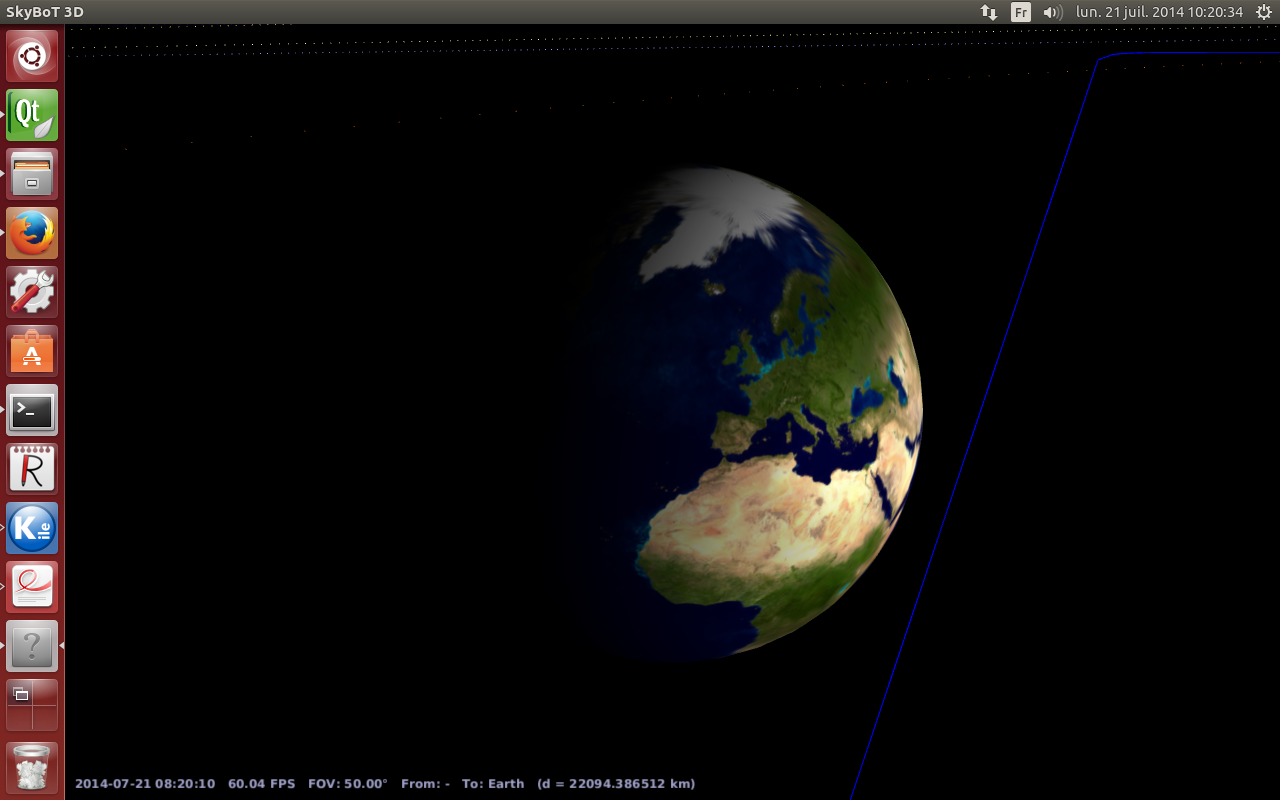
\includegraphics[width=1.0\textwidth]{skybot_normal_earth.png}
			      \caption{Visualisation de la planète Terre dans Skybot 3D en vue normale}
		\end{figure}
		
		\begin{figure}
			      \centering
			      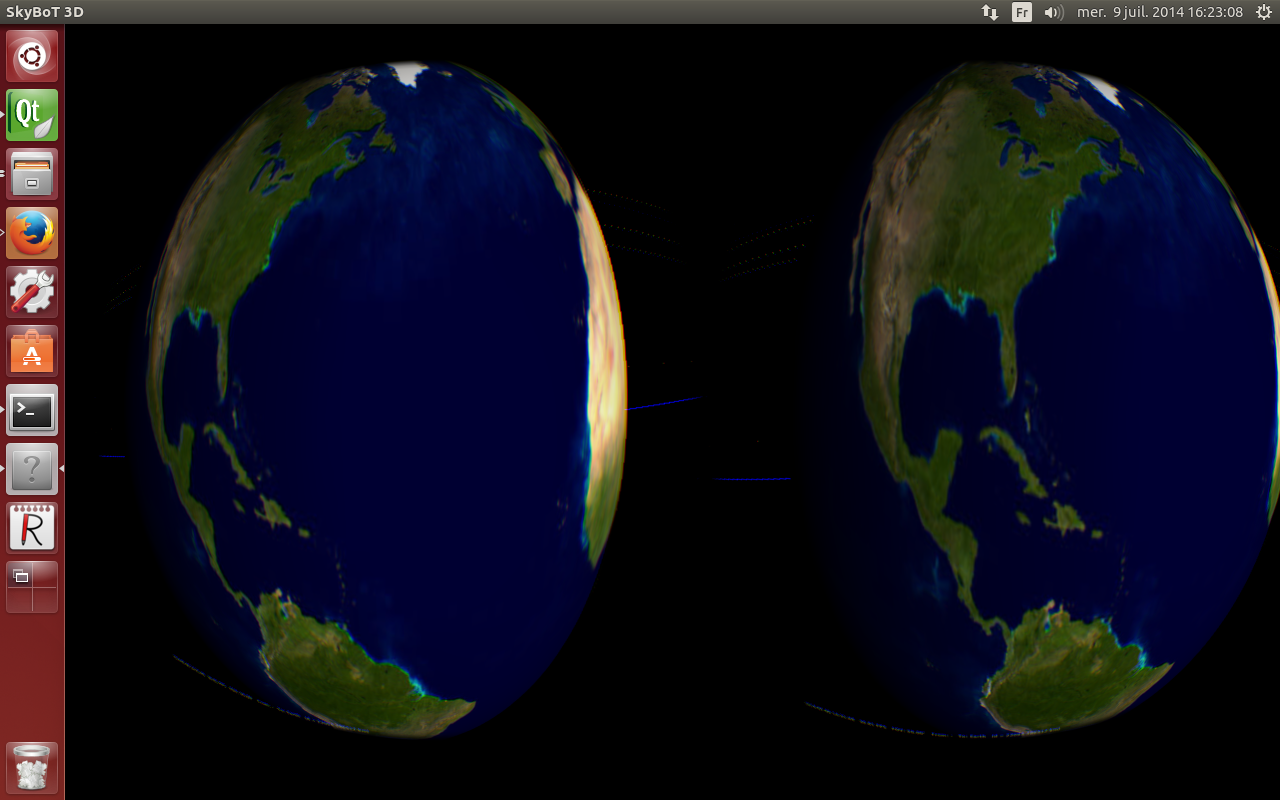
\includegraphics[width=1.0\textwidth]{skybot_oculus_earth.png}
			      \caption{Visualisation de la planète Terre dans Skybot 3D en vue Oculus}
		\end{figure}
		
		\begin{figure}
			      \centering
			      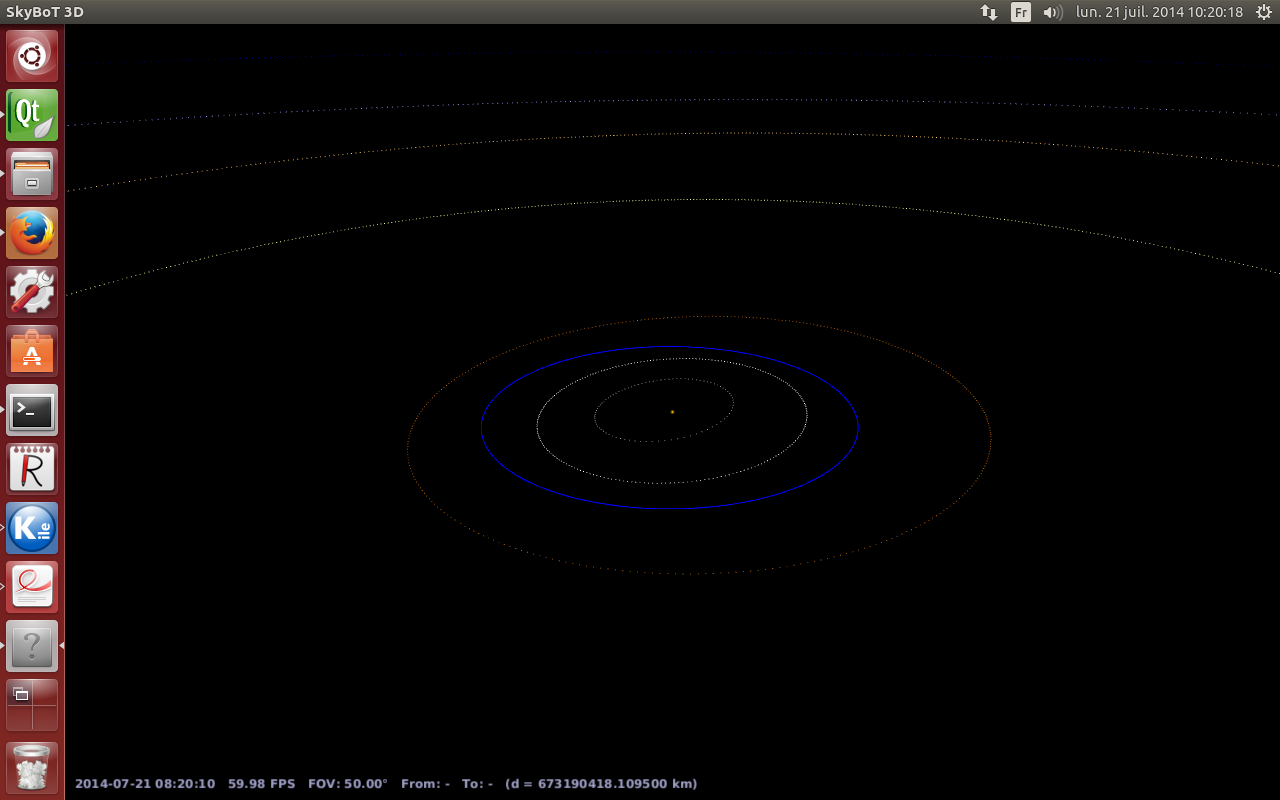
\includegraphics[width=1.0\textwidth]{skybot_normal.png}
			      \caption{Visualisation du systême solaire dans Skybot 3D en vue normale}
		\end{figure}
		
		\begin{figure}
			      \centering
			      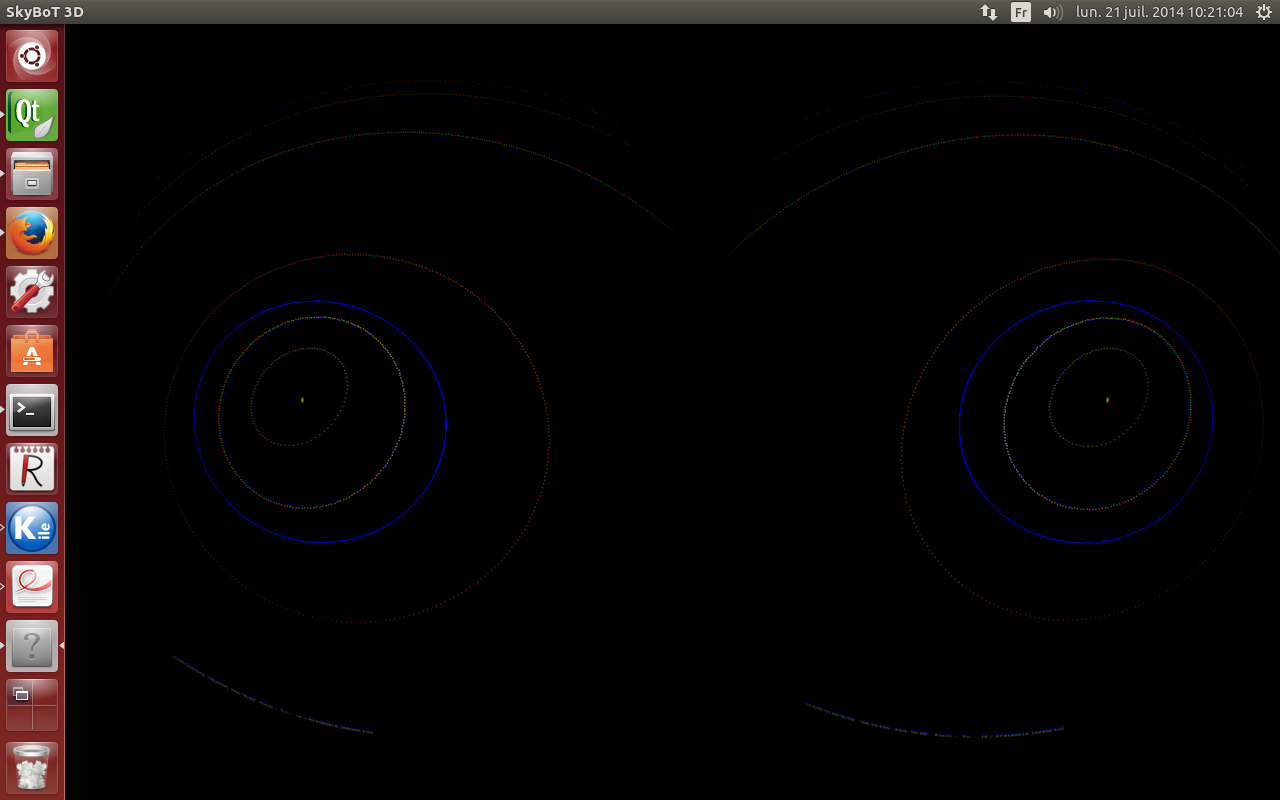
\includegraphics[width=1.0\textwidth]{skybot_oculus.png}
			      \caption{Visualisation du systême solaire dans Skybot 3D en vue Oculus}
		\end{figure}
		
		\FloatBarrier
		Les images suivantes présentent l'application de simulation d'un cube de données d'objets célestes, 
		organisés en un Octree  de taille 128*128*128, divisé en octants de taille 8.
		
		Les objets céleste sont modélisés par des cubes texturés de taille 1.
		
		Seul l'octant actuel et les octants directement voisins sont visibles pour des raisons de performances.
		
		La caméra est dirigeable par les mouvements de la tête en mode Oculus.
		
		
		\begin{figure}
			      \centering
			      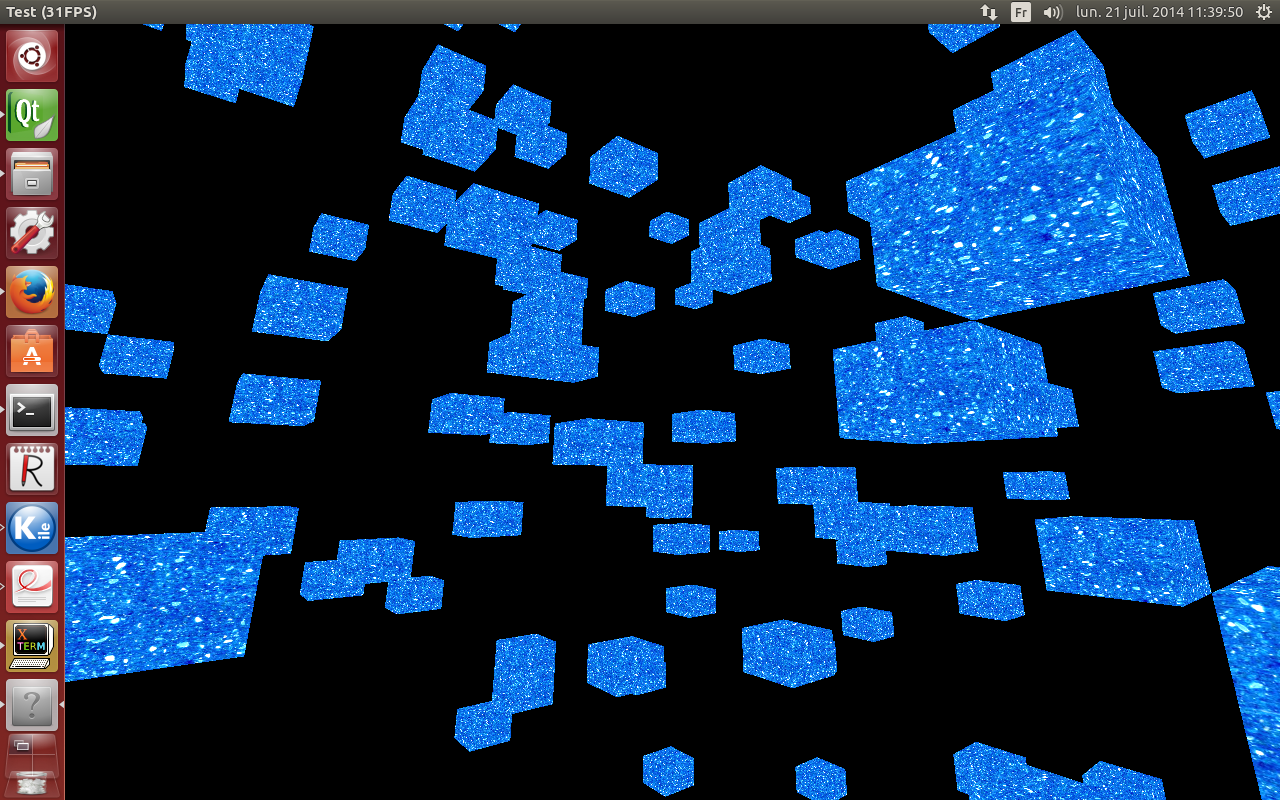
\includegraphics[width=1.0\textwidth]{octree_normal.png}
			      \caption{Simulation en vue normale}
		\end{figure}
		
		\begin{figure}
			      \centering
			      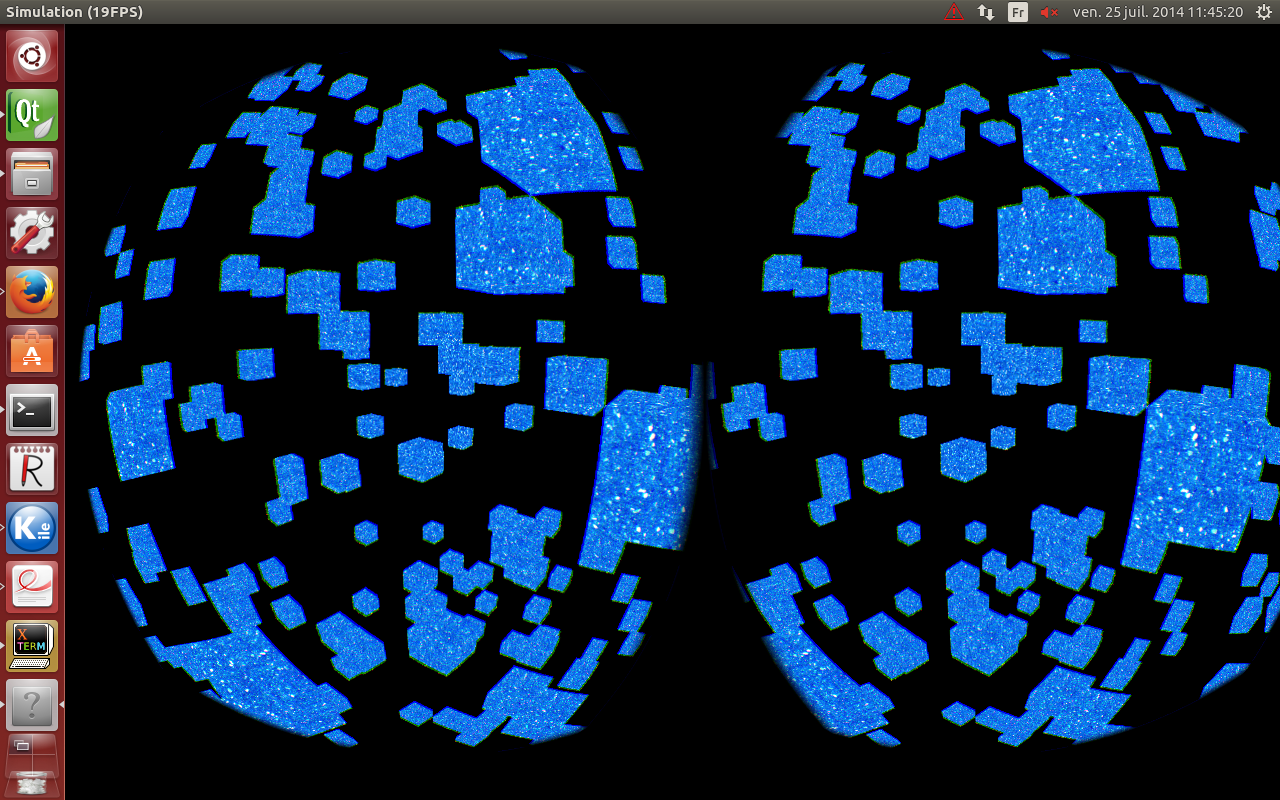
\includegraphics[width=1.0\textwidth]{octree_oculus.png}
			      \caption{Simulation en vue normale}
		\end{figure}
		\FloatBarrier
		
		Les images suivantes présentent l'application de simulation d'un cube de données d'objets célestes, 
		organisés en un tableau simple.
		
		Les objets céleste sont modélisés par des cubes texturés de taille 1.
		
		\begin{figure}
			      \centering
			      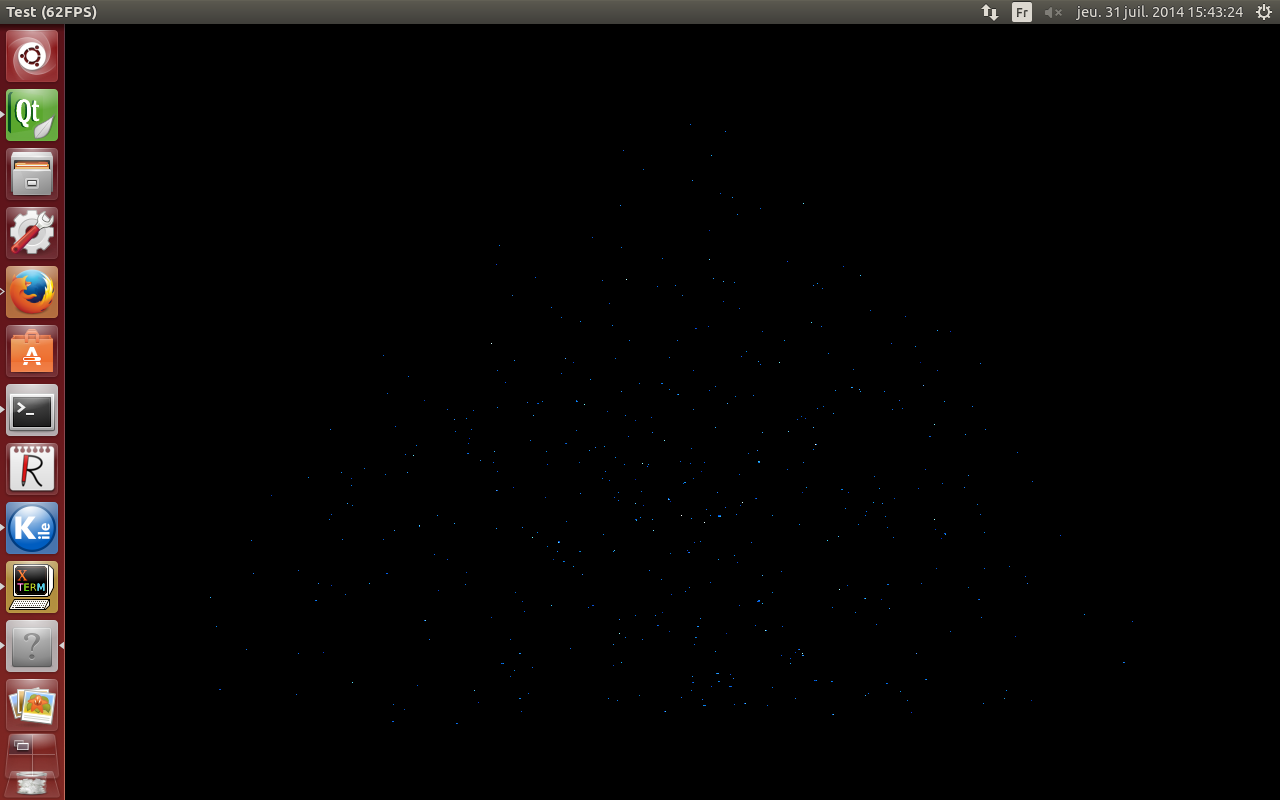
\includegraphics[width=1.0\textwidth]{basic_normal.png}
			      \caption{Simulation en vue normale}
		\end{figure}
		
		\begin{figure}
			      \centering
			      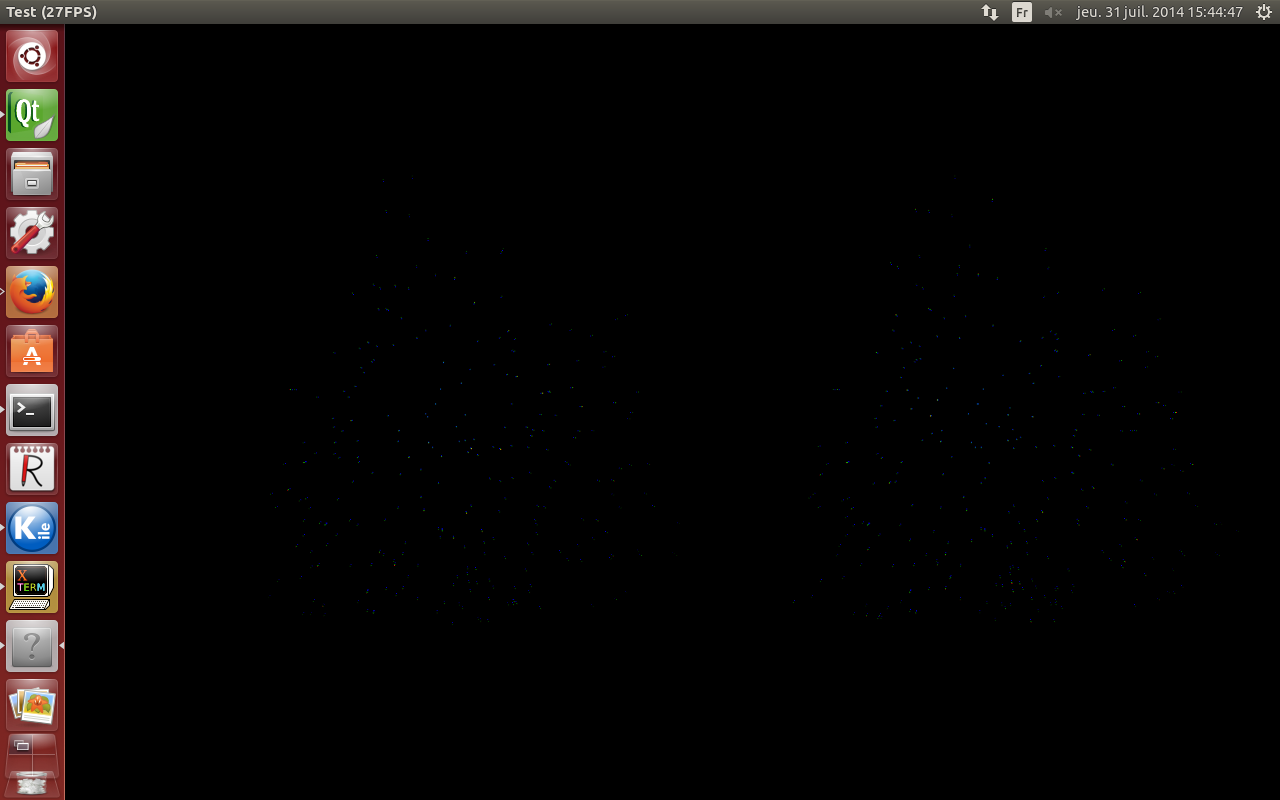
\includegraphics[width=1.0\textwidth]{basic_oculus.png}
			      \caption{Simulation en vue normale}
		\end{figure}
		\FloatBarrier
		
	\newpage	
	\subsection{Code source}
	\epigraph{Talk is cheap. Show me the code}{Linus Torvalds}
	
	\FloatBarrier
	<<Oculus.h>> est un fichier d'en-tête décrivant la classe Oculus. Il prend comme argument de template la scene
	OpenGL générique que l'on veut afficher en mode Oculus. La seule contrainte est que cette scène fournisse 
	la méthode <<render>>.
	\lstinputlisting[language=C++]{Oculus.h}
	\FloatBarrier
		
	\subsection{Glossaire}
		\begin{description}
		
		\item [API]~\\
		    <<Application Programming Interface>>, interface de programmation. Ensemble normalisé de classes et de 
		    fonctions qui sert de façade par laquelle un logiciel offre des services à d'autres logiciels.
		
		\item [C] ~\\
		    Langage de programmation impératif, procédural utilisé dans des applications ayant un besoin critique
		    de performances.
		    
		\item [C++] ~\\
		    Langage de programmation mutliplateforme, multiparadigme, générique, compilé, largement utilisé
		    dans les domaines scientifiques, industriels, de l'entreprise, de l'image, \ldots
		
		\item [CPU]~\\
		    <<Central Processing Unit>>, processeur. 
		    Composant de l'ordinateur qui exécute les instructions machine des programmes informatiques.
		
		\item [FPS] ~\\
		      <<Frame Per Seconds>>, mesure de la fluidité du rendu graphique en images par seconde.
		
		\item [Frame]~\\
		    Image rendue graphiquement par un programme, typiquement 60 fois par seconde.
		    
		\item [Framework]~\\
		    Ensemble cohérent de composants logiciels structurels.

		\item [GPU]~\\
		    <<Graphics Processing Unit>>, processeur graphique.
		    Circuit intégré présent sur une carte graphique et assurant les fonctions de calcul de l'affichage.
		
		\item [Oculus Rift]~\\
		    Masque de réalité virtuelle fournissant une expérience d'immersion inédite.
		    
		\item [Oculus VR]~\\
		    Entreprise de réalité virtuelle fabriquant l'Oculus Rift.
		    
		
		\item [SDK]~\\
		    <<Software Develoment Kit>>, kit de développement. 
		    Ensemble d'outils permettant aux développeurs de créer des applications de type défini.
		    
		\item [Shader]~\\
		    Programme informatique, utilisé en image de synthèse, 
		    pour paramétrer une partie du processus de rendu réalisé par une carte graphique ou un moteur de rendu logiciel.
		    Ils peuvent permettre de décrire l'absorption et la diffusion de la lumière, la texture à utiliser, 
		    les réflexions et réfractions, l'ombrage, le déplacement de primitives 
		    et des effets post-traitement. 

		\end{description}

	\subsection{Ressources}
	  \begin{description}
	  \item [Site web du créateur du langage C++]~\\
	      \url{http://www.stroustrup.com/}
	  \item [Conventions de code C++]~\\
	      \url{http://www.stroustrup.com/JSF-AV-rules.pdf}
	  \item [Site d'Oculus pour les développeurs]~\\
	      \url{https://developer.oculusvr.com/}
	  \item [Wiki officiel d'OpenGL]~\\
	      \url{http://www.opengl.org/wiki/Main_Page}
	  \item [Site web sur les design patterns]~\\
	      \url{http://gameprogrammingpatterns.com/}
	  \item [Blog sur le développement Oculus Rift]~\\
	      \url{http://rifty-business.blogspot.fr}
	  \item [Tutoriel C++]~\\
	      \url{http://cpp.developpez.com/faq/cpp/}
	  \item [Tutoriel OpenGL 3.x]~\\
	      \url{http://tomdalling.com/blog/category/modern-opengl/}  
	  \item [Site web de Skybot 3D]~\\
	      \url{http://vo.imcce.fr/webservices/skybot3d}  
	  \item [Site web de l'Observatoire]~\\
	      \url{http://astro.unistra.fr/}  
	  \item [Site web traitant du problème d'échelle et des grands nombres dans OpenGL]~\\
	      \url{http://www.floatingorigin.com/}  
	  \item [Autre tutoriel OpenGL 3.x]~\\
	      \url{http://open.gl/}  
	  \item [Oculus SDK]~\\
	      \url{https://developer.oculusvr.com/?action=dl}  
	  \item [Page Github du projet de Simulation]~\\
	    \url{https://github.com/gaultier/Simulation_Stage_2014}
	  \end{description}

	
	
\end{document}

